% !TEX root = perelman-geometry.tex
%!TEX TS-program = pdflatex
%!TEX encoding = UTF-8 Unicode



\setchapterpreamble[o]{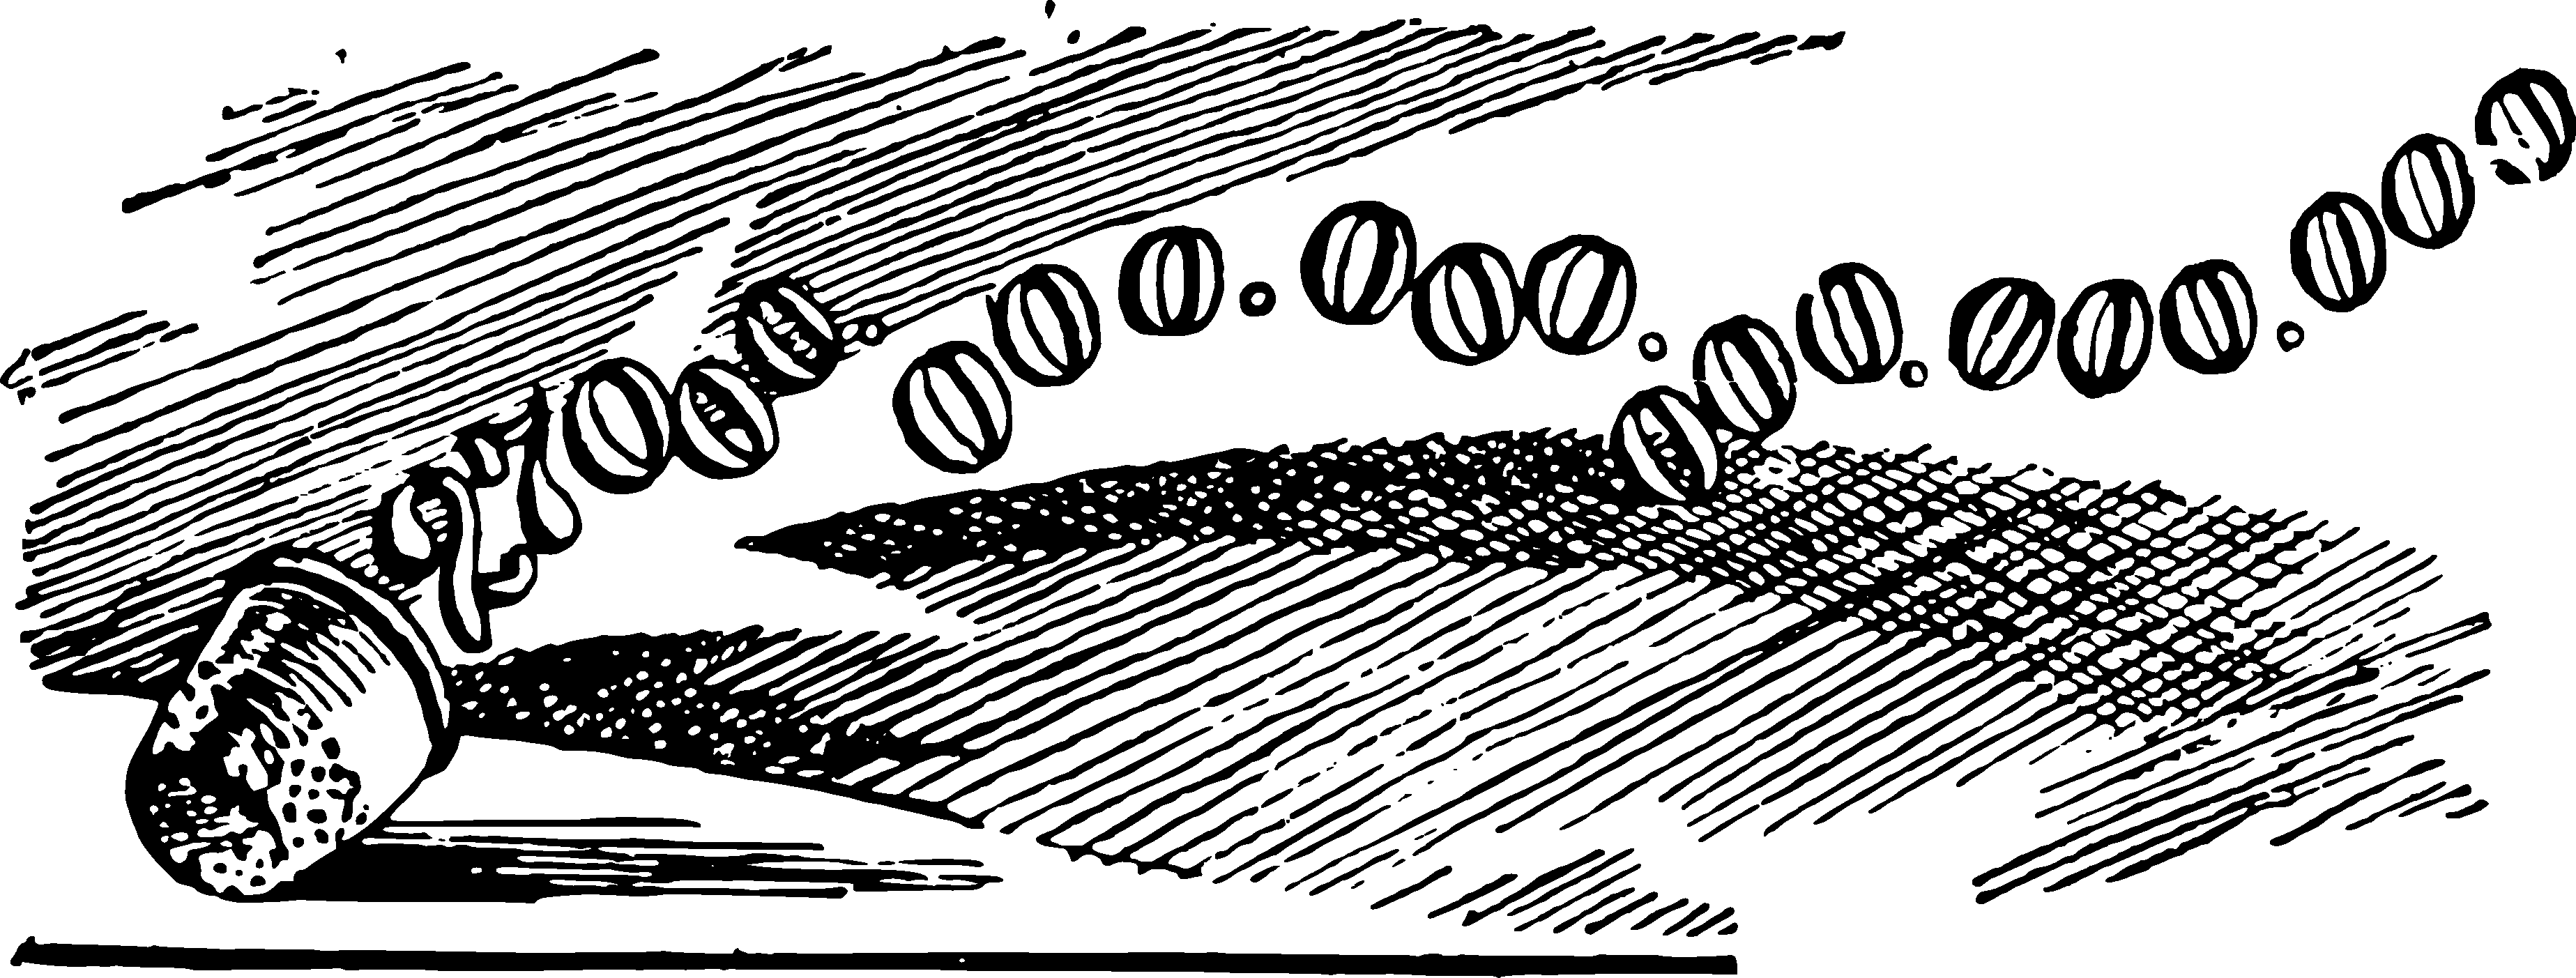
\includegraphics[width=1.2\textwidth]{figures/ch-11/fig-ch-11-head.pdf}\bigskip}

\chapter{Big And Small In Geometry}
\label{ch-11}



\section{In a Thimble}\marginnote{\large \num{21000000000000000000}}
\label{sec-11.1}

The number twenty-seven with eighteen zeros, written in the margin, can be read in different ways. Some will say: this is 27 trillion; others, for example financial workers, will read it as 27 quintillion, and still others will write it shorter: \num{27d18} and read it as 27 multiplied by ten to the eighteenth power.

But what can fit in such an incredible quantity in one thimble?

We are talking about particles of the air surrounding us. Like all substances in the world, air consists of molecules. Physicists have established that in every cubic centimetre (i.e., approximately in a thimble) of the air surrounding us at a temperature of \SI{0}{\degreeCelsius}, there are 27 trillion molecules. This is a numerical giant. To imagine it in any meaningful way is beyond the ability of even the liveliest imagination. Indeed, what can be compared to such a multitude? To the number of people in the world? But there are ``only'' two billion people on the globe (\num{2d9}), which is thirteen thousand million times smaller than the number of molecules in a thimble. 

Even if all the stars in the universe, visible to the most powerful telescope, were surrounded by planets like our Sun, and if each of these planets were inhabited as our Earth is, then even the number of inhabitants would not equal the molecular population of one thimble! If you attempted to count this invisible population, counting continuously, for example, at a rate of a hundred molecules per minute, it would take you at least five hundred billion years to count.

\begin{figure}[h!]
\centering
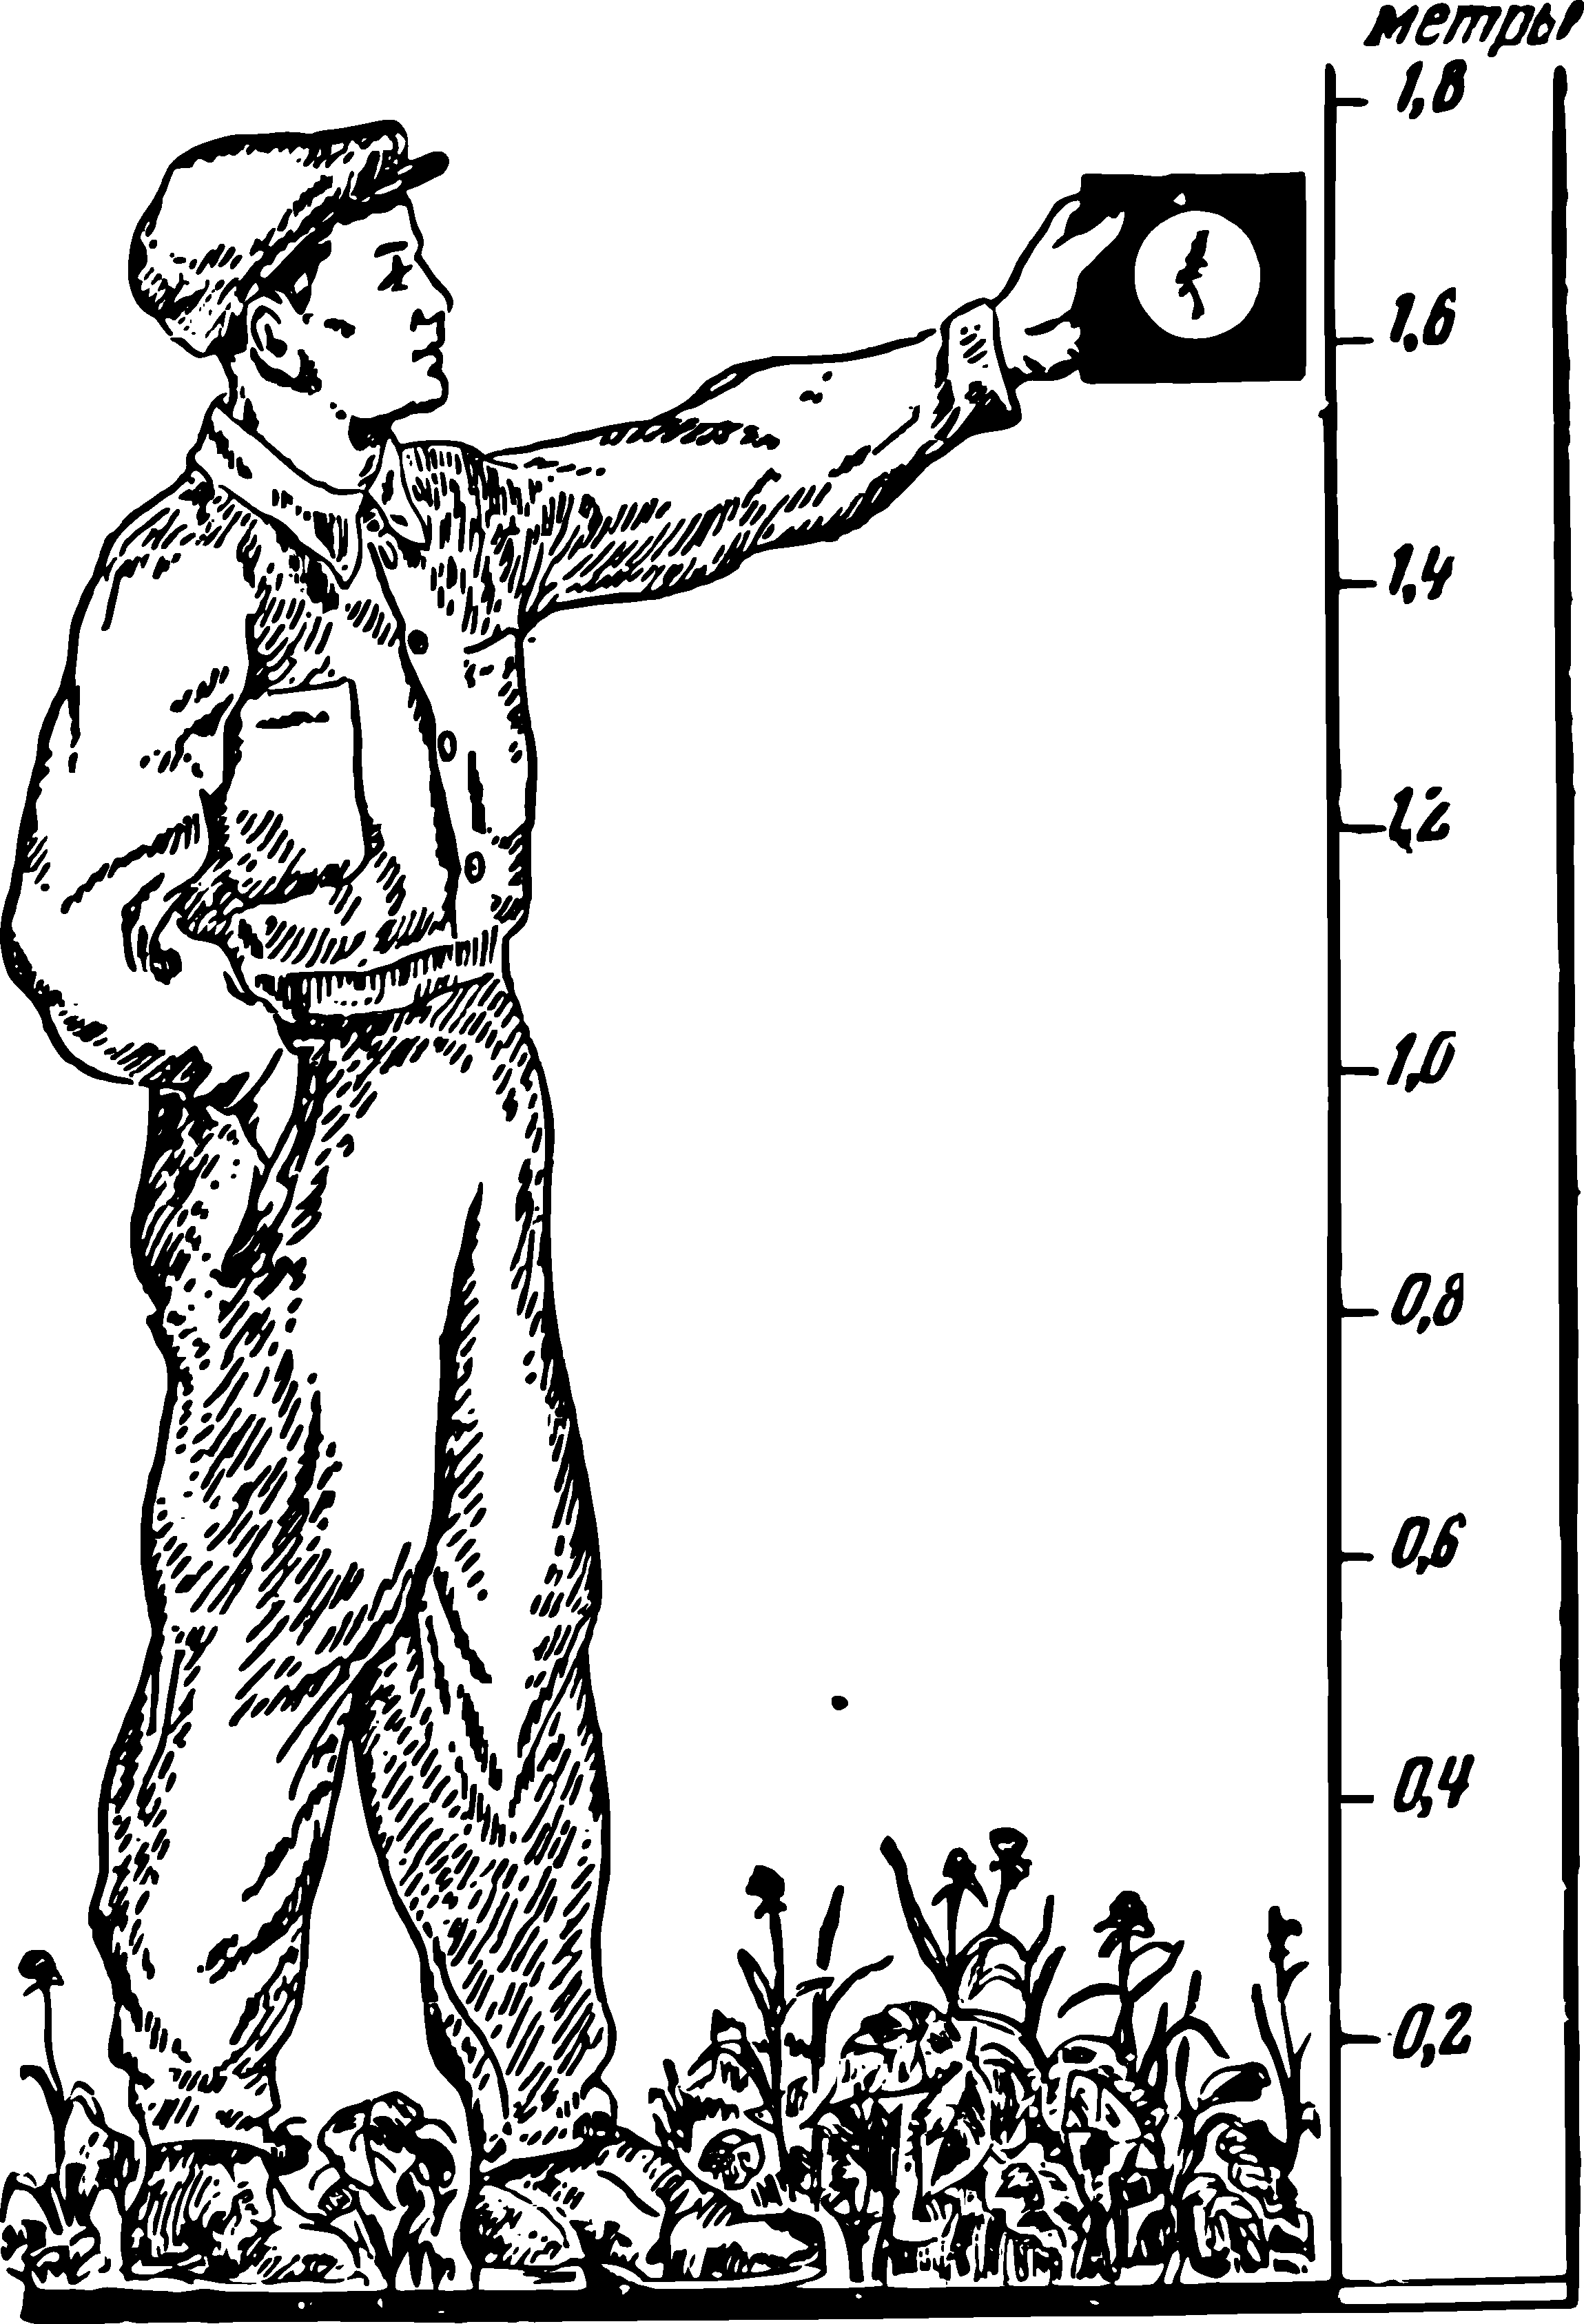
\includegraphics[width=0.6\textwidth]{figures/ch-11/fig-160.pdf}
\sidecaption{The young man looks at the typhus bacillus, magnified 1000 times.\label{fig-160}}
\end{figure}

Not everyone can clearly imagine even more modest numbers.

What do you envision when you are told, for example, about a microscope that magnifies by 1000 times? Not such a large number, just a thousand, but nevertheless, a thousandfold magnification is not perceived by everyone as it should be. We often fail to appreciate the true smallness of the objects we see under a microscope at such magnification. A typhoid bacterium, magnified by 1000 times, seems to us the size of a fly (see \figr{fig-160}) viewed at a distance of clear vision, i.e., \SI{25}{\centi\meter}. 


But how small is this bacterium really? Imagine that along with the magnification of the bacterium, you also magnified yourself by 1000 times. This means that your height would reach 1700 m! Your head would be above the clouds, and any of the new skyscrapers being built in Moscow would seem much lower than your knees (see \figr{fig-160}). The bacterium is as much smaller than the tiny fly as you are smaller than this imaginary giant.

\begin{figure}[h!]
\centering
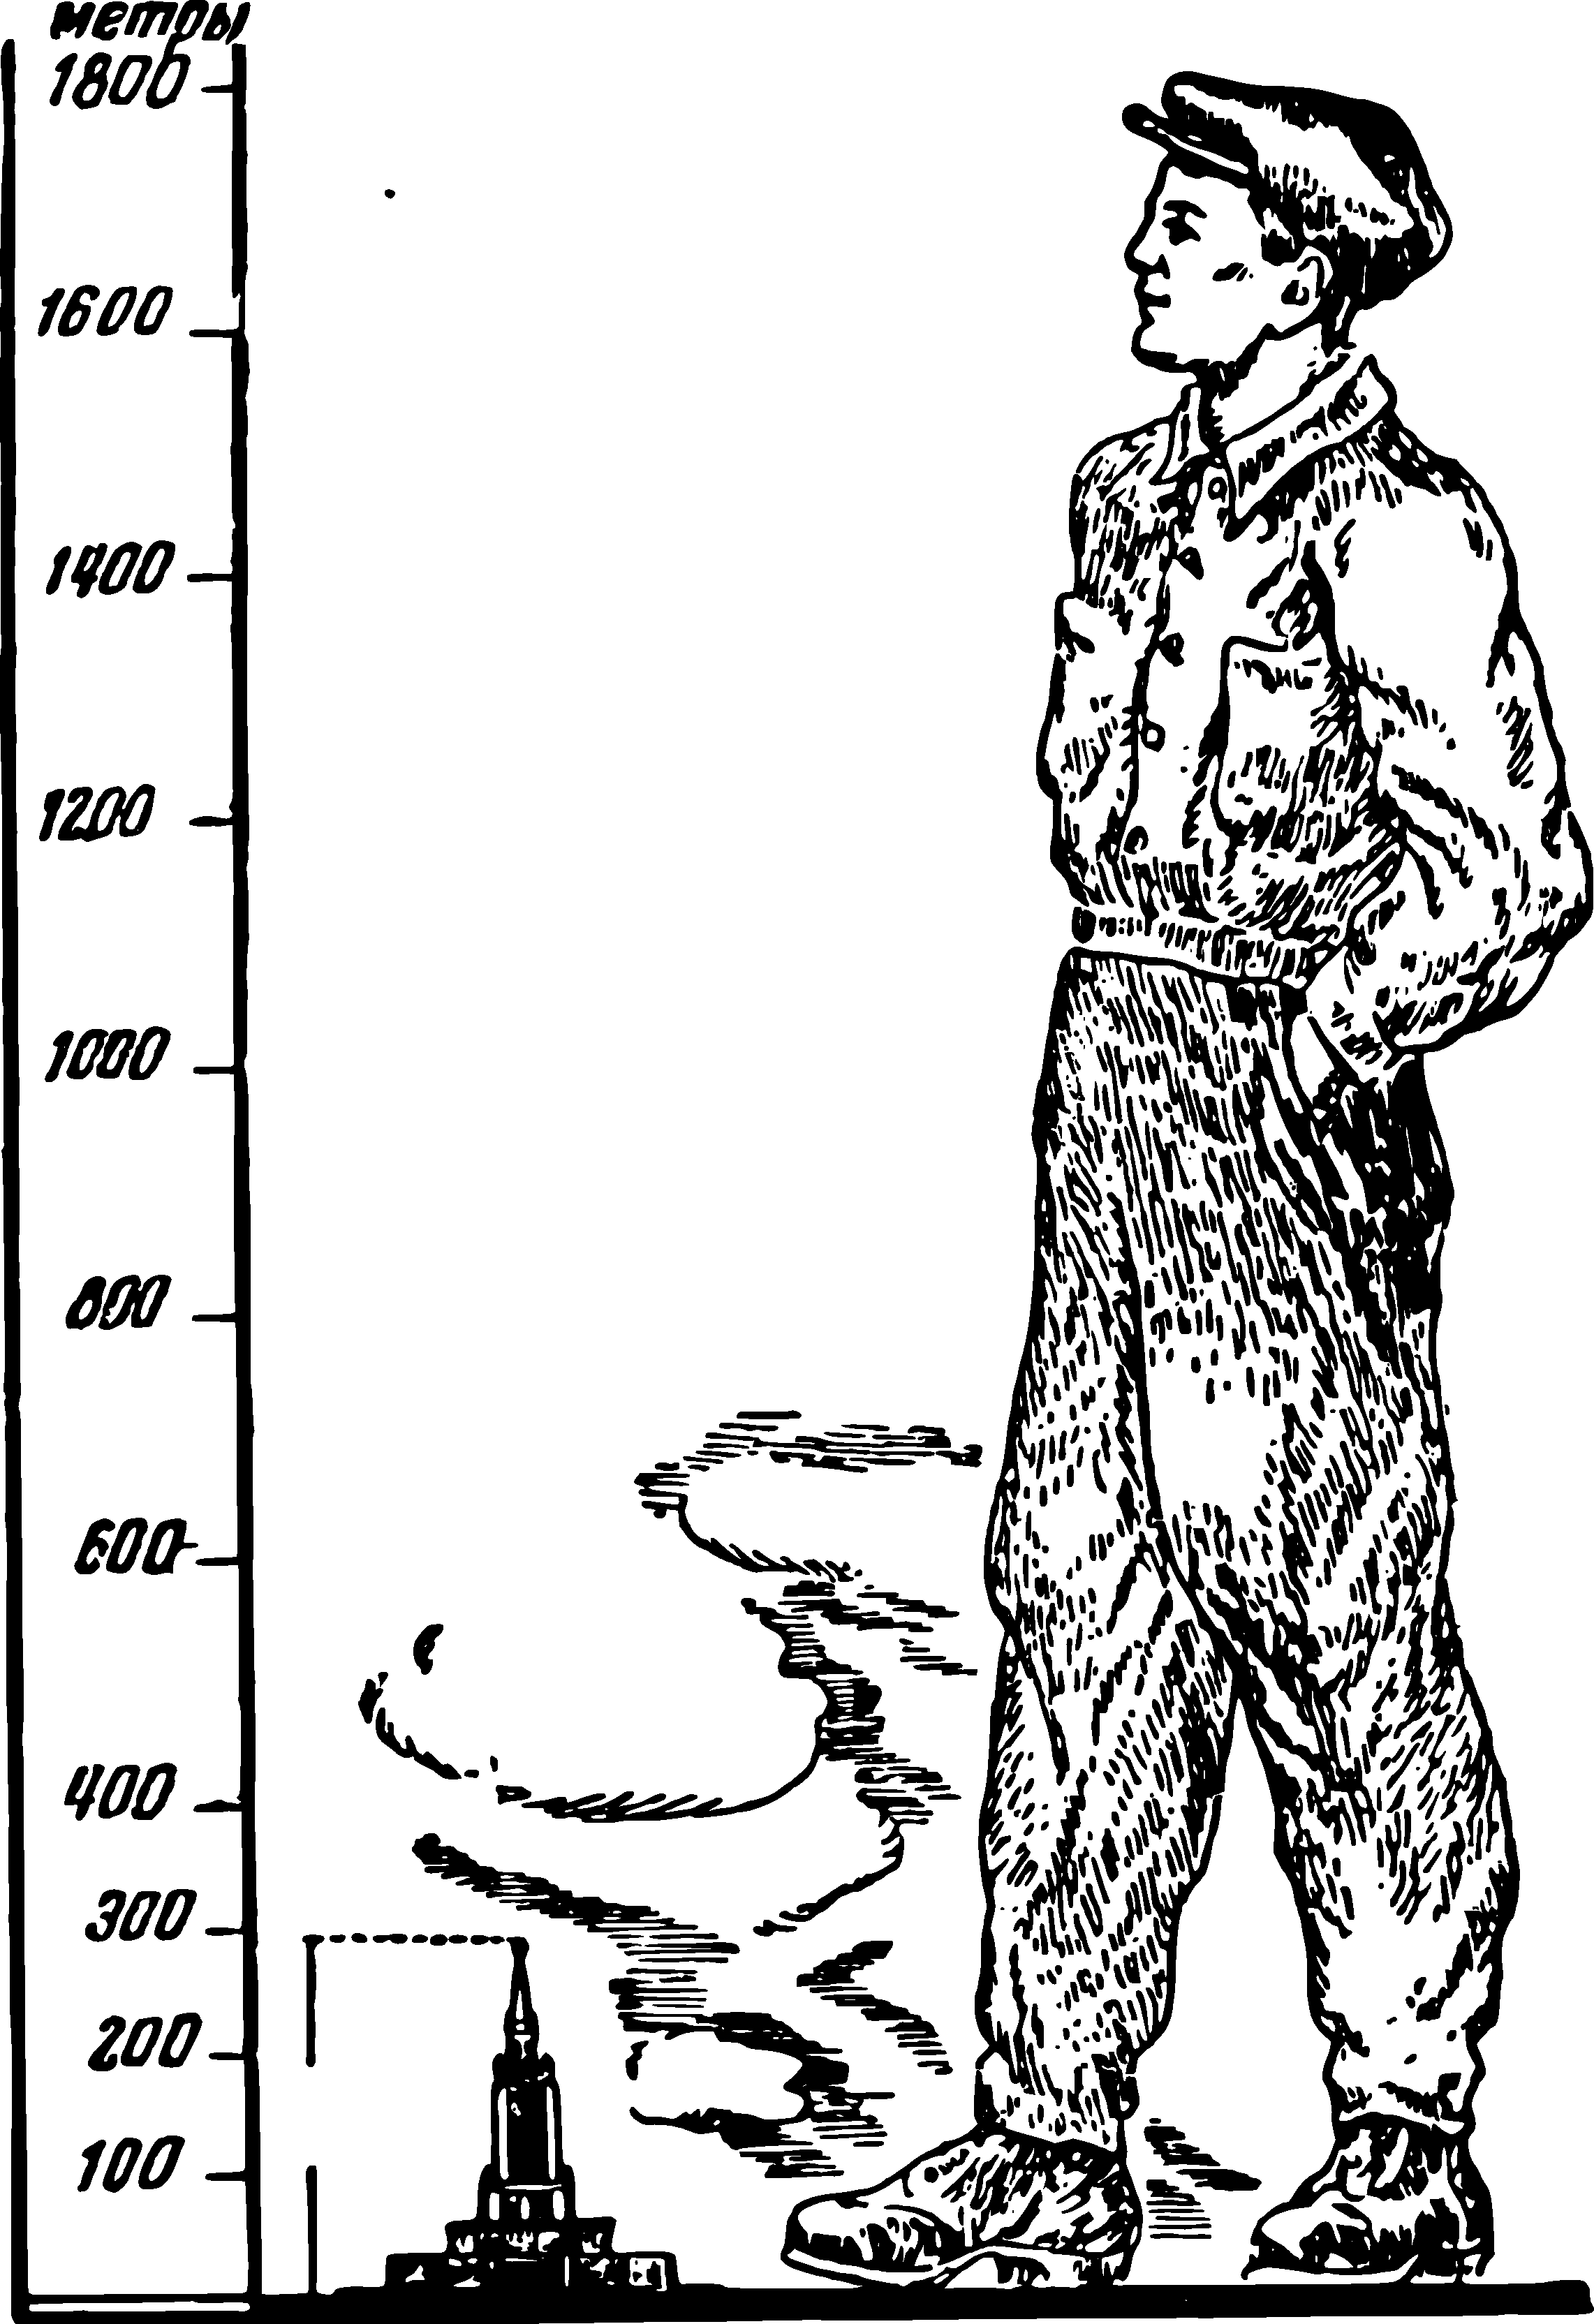
\includegraphics[width=0.6\textwidth]{figures/ch-11/fig-161.pdf}
\sidecaption{A young man magnified 1000 times.\label{fig-161}}
\end{figure}


\section{Volume and Pressure}
\label{sec-11.2}

One might think -- isn’t it too cramped for 27 trillion air molecules in a thimble? Not at all! An oxygen or nitrogen molecule has a diameter of 3/10,000,000 mm (or \SI{3d-7}{\milli\meter}). If we assume the volume of a molecule to be the cube of its diameter, we get:
\begin{equation*}%
\left( \frac{3}{10^{7}} \si{\milli\meter} \right)^3 = \frac{27}{\num{d21}} \,\si{\milli\meter\cubed}.
\end{equation*}
There are \num{27d18} molecules in a thimble. Thus, the volume occupied by all the inhabitants is approximately:
\begin{equation*}%
\frac{27}{10^{21}} \times 27 \times 10^{18} = \frac{729}{10^3} \,\si{\milli\meter\cubed}
\end{equation*}
That is, about \SI{1}{\milli\meter\cubed}, which constitutes only one-thousandth of a cubic centimetre. The gaps between the molecules are many times larger than their diameters, so there is plenty of space for the molecules to move around. Indeed, as you know, air particles do not lie still, clustered together, but continuously and chaotically move from place to place, traversing the space they occupy. Oxygen, carbon dioxide, hydrogen, nitrogen, and other gases have industrial significance, but storing them in large quantities would require enormous reservoirs. For example, one ton (1000 kg) of nitrogen at normal pressure occupies a volume of 800 cubic meters, which means that to store just one ton of pure nitrogen, you would need a box measuring $\SI{20}{\meter} \times \SI{20}{\meter} \times \SI{20}{\meter}$. And to store one ton of pure hydrogen, a tank with a capacity of 10,000 cubic meters would be needed.

Can we make gas molecules squeeze together? Engineers do just that —- by compressing them, they force the molecules to become denser. But this is not an easy task. Don't forget that the pressure applied to the gas is met with equal force exerted by the gas on the vessel walls. Very strong walls are needed, which are also chemically resistant to the gas.

Modern chemical apparatus, manufactured domestically from alloy steels, can withstand enormous pressures, high temperatures, and the harmful chemical effects of gases.

Today, our engineers compress hydrogen to 1163 times its original density, so that one ton of hydrogen, which at atmospheric pressure occupies a volume of 10,000 cubic meters, fits into a relatively small cylinder with a capacity of about 9 cubic meters (see \figr{fig-162}).


\begin{figure}[h!]
\centering
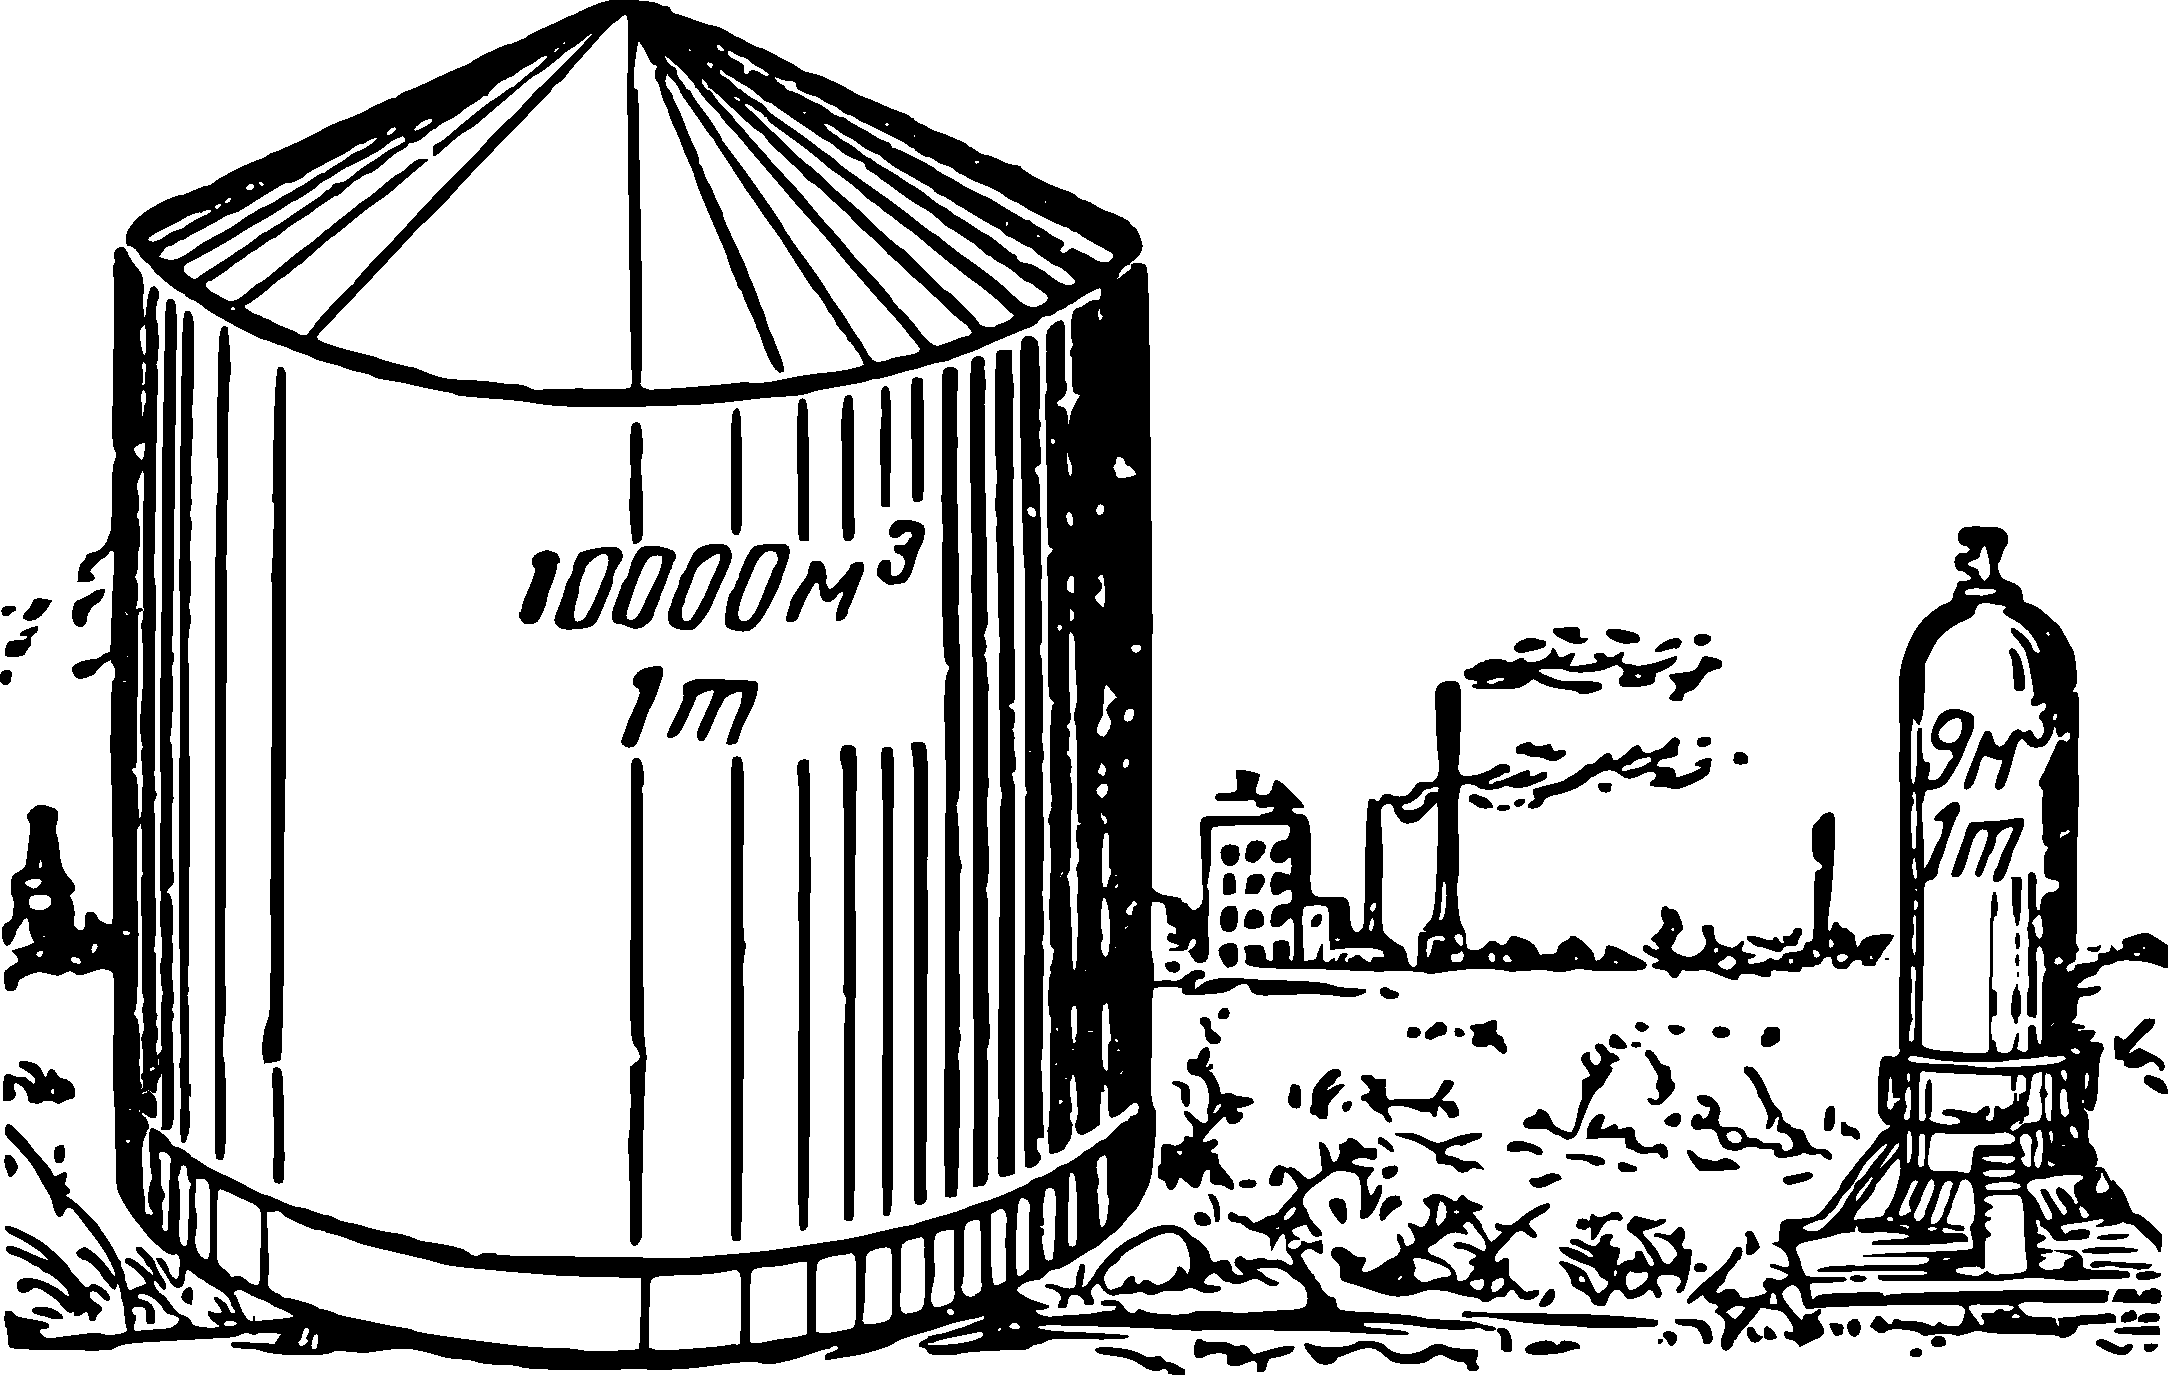
\includegraphics[width=0.8\textwidth]{figures/ch-11/fig-162.pdf}
\sidecaption{A ton of hydrogen at atmospheric pressure (to the left) and at a pressure of 5,000 atm (to the right). (The drawing is not to scale.)\label{fig-162}}
\end{figure}


How do you think hydrogen was subjected to reduce its volume by 1163 times? Recalling from physics that the volume of gas decreases proportionally to the increase in pressure, you might suggest this answer: the pressure on the hydrogen was increased by 1163 times. Is that actually the case? No. In reality, hydrogen had to be subjected to a pressure of 5000 atmospheres, i.e., the pressure was increased by 5000 times, not 1163 times. The fact is, this proportionality only holds for relatively low pressures.

At very high pressures, this relationship does not apply. For example, when one ton of nitrogen at our chemical plants is subjected to a pressure of 1000 atmospheres, the entire ton fits into a volume of 1.7 cubic meters instead of the 800 cubic meters it occupies at normal atmospheric pressure. Moreover, when the pressure is further increased to 5000 atmospheres, or five times, the volume of nitrogen decreases to just 1.1 cubic meters.



\section{Thinner than a spider web but stronger than steel}
\label{sec-11.3}

The cross-section of a thread, wire, or even a spider web, no matter how small, still has a definite geometric shape, most often a circle. The diameter of the cross-section, or let's say, the thickness of a single spider web is about 5 microns (5/1000 mm). Is there anything thinner than a spider web? Who is the most skilled ``thin-spinner''? The spider or perhaps the silkworm? No. The diameter of a natural silk thread is 18 microns, meaning the thread is 3.5 times thicker than a spider web.

People have long dreamt of surpassing the craftsmanship of the spider and the silkworm. There is an ancient legend about a marvellous weaver, the Greek Arachne\sidenote{Arachne is the protagonist of a tale in Greek mythology known primarily from the version told by the Roman poet Ovid. -- \textsc{dm}}.

She mastered the weaving craft so perfectly that her fabrics were as fine as a spider web, transparent as glass, and light as air. Even the goddess Athena -- the goddess of wisdom and patron of crafts -- could not compete with her.

This legend, like many other ancient myths and fantasies, has become reality in our time. The modern Arachne, the most skilled ``thin-spinner'', turned out to be chemical engineers who created an extraordinarily thin and remarkably strong artificial fibre from ordinary wood. Silk threads produced by the copper-ammonia industrial method, for example, are 2.5 times thinner than a spider web and almost as strong as natural silk threads. Natural silk can withstand a load of up to 30 kg per square mm of cross-section, while copper-ammonia silk can withstand up to 25 kg per square mm.


A curious method of producing copper-ammonia silk involves transforming wood into cellulose, then dissolving the cellulose in an ammonia solution of copper. Streams of this solution are extruded through fine openings into water, which removes the solvent. The resulting fibres are then wound onto appropriate devices. The thickness of copper-ammonia silk thread is 2 microns. One micron thicker is the so-called acetate silk, which is also artificial. Remarkably, some types of acetate silk are stronger than steel wire! If steel wire can withstand a load of 110 kg per square millimetre of cross-section, acetate silk thread can withstand 126 kg per square millimetre.


\begin{figure}[h!]
\centering
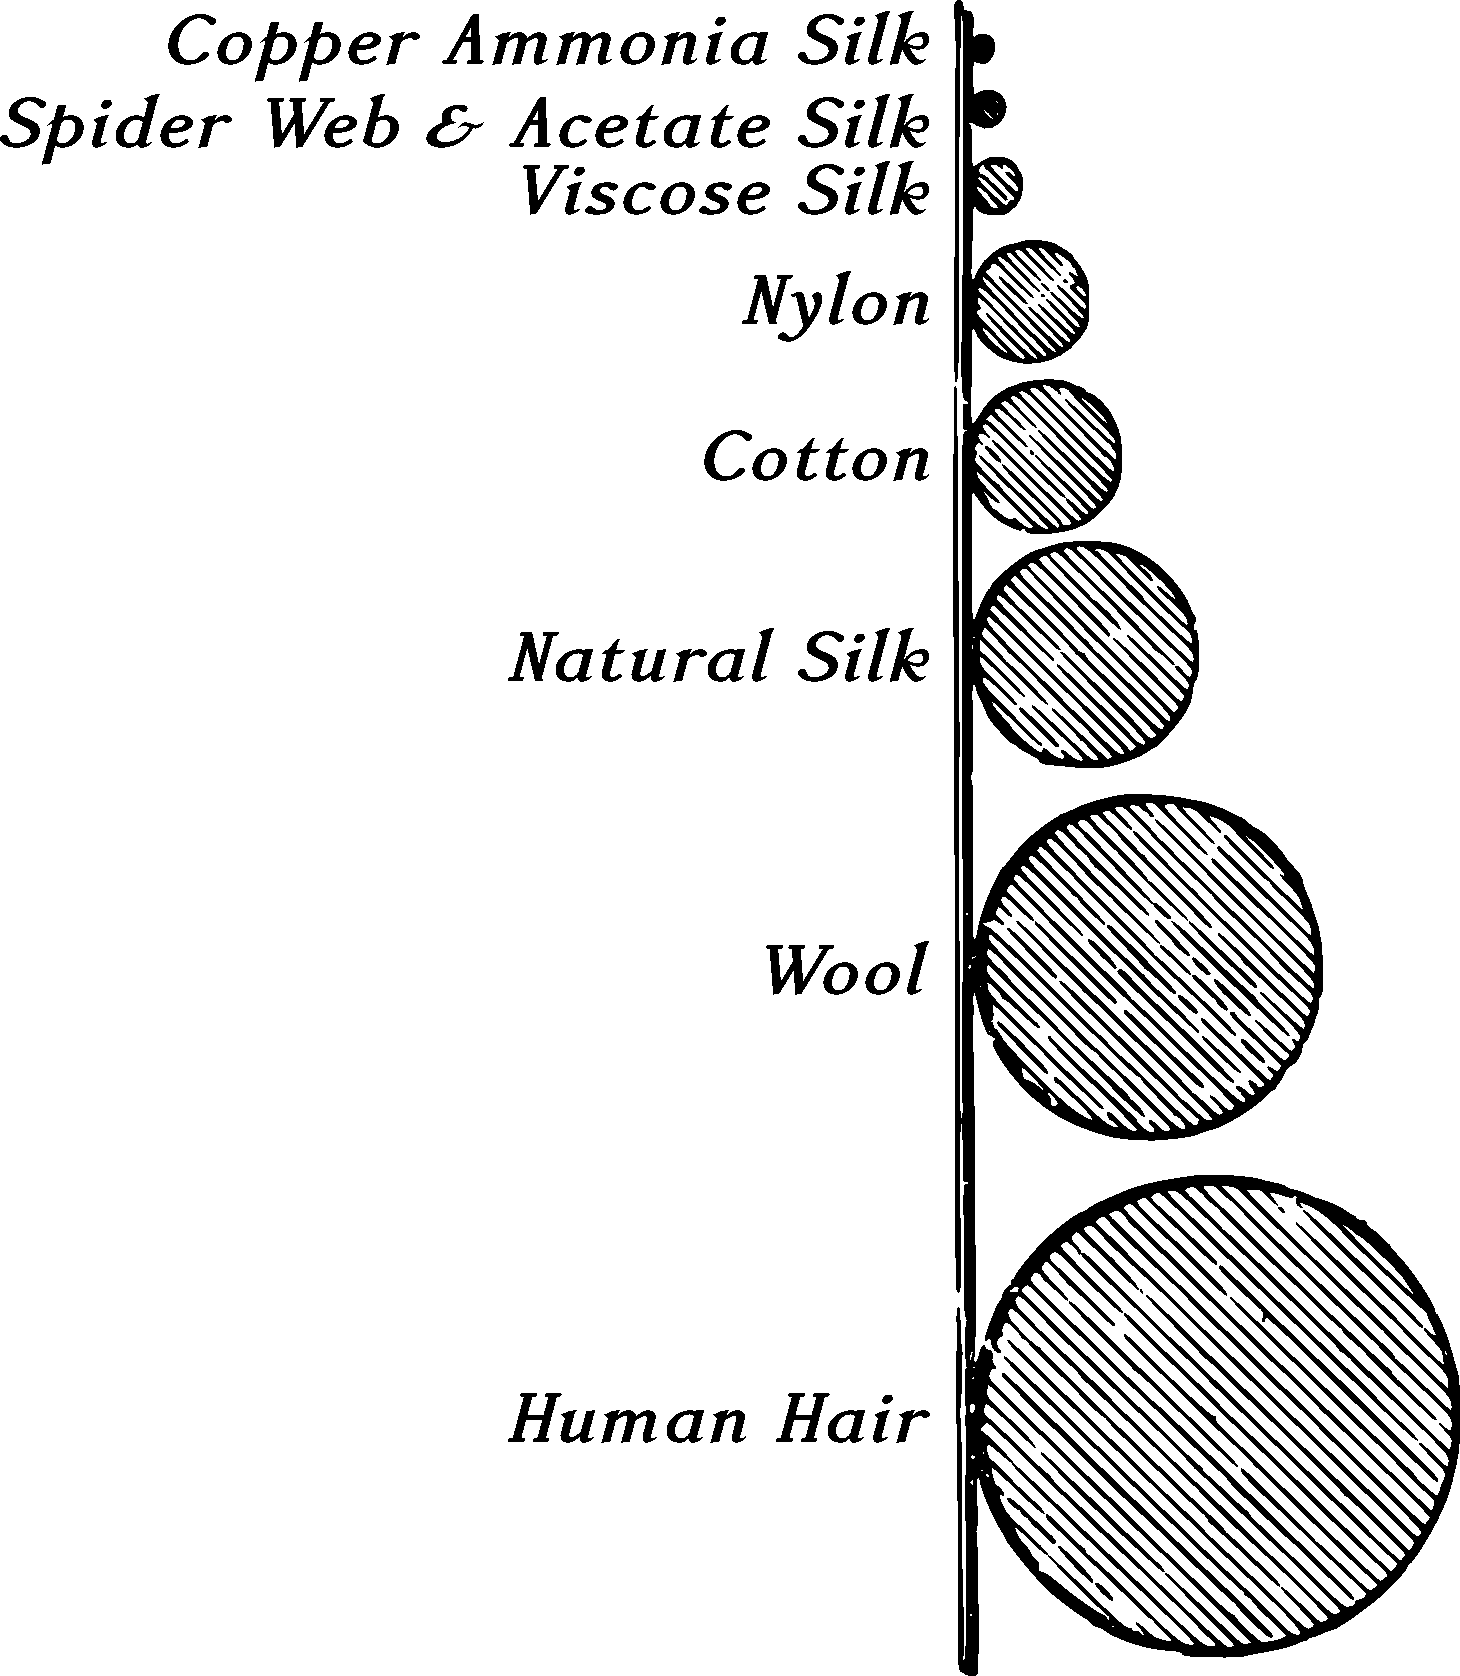
\includegraphics[width=0.7\textwidth]{figures/ch-11/fig-163a.pdf}
\sidecaption{The comparative thickness of the fibres.\label{fig-163}}
\end{figure}



The well-known viscose silk has a thread thickness of about 4 microns and a tensile strength ranging from 20 to 62 kg per square millimetre of cross-section. \figr{fig-163} shows the comparative thicknesses of spider silk, human hair, various artificial fibres, as well as wool and cotton fibres, while \figr{fig-164} illustrates their strength in kilogrammes per square millimetre. Artificial, or synthetic, fibre is one of the major modern technological discoveries and has significant economic importance. Engineer Buyanov shares the following:
\begin{quote}
Cotton grows slowly, and its quantity depends on climate and harvest. The producer of natural silk, the silkworm, is extremely limited in its capabilities. Throughout its life, it spins a cocoon containing only 0.5 grams of silk thread \dots{}

The amount of artificial silk obtained through chemical processing from 1 cubic meter of wood can replace 320,000 silk cocoons or the annual wool yield from 30 sheep, or the average cotton harvest from half a hectare. This quantity of fibre is sufficient to produce four thousand pairs of women's stockings or 1500 meters of silk fabric.
\end{quote}
\begin{figure}[h!]
\centering
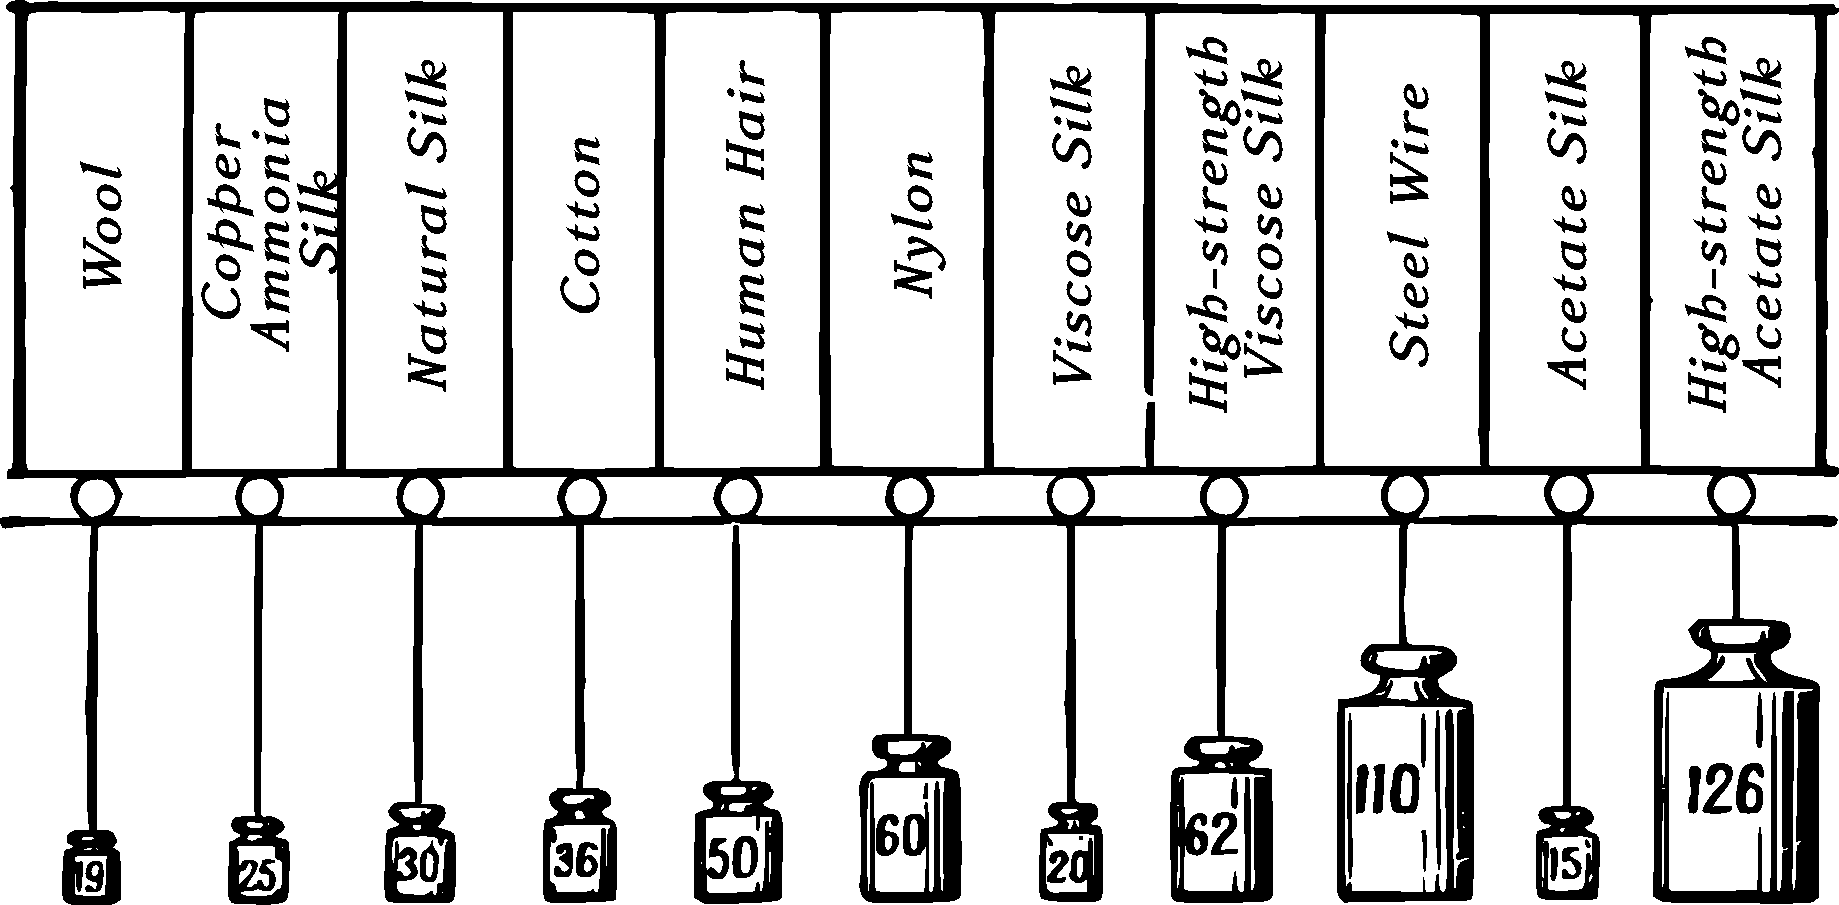
\includegraphics[width=0.9\textwidth]{figures/ch-11/fig-164a.pdf}
\sidecaption{The ultimate strength of fibres (in kg per 1 sq. m of cross section)\label{fig-164}}
\end{figure}





\section{Two Jars}
\label{sec-11.4}



We have an even poorer understanding of large and small quantities in geometry, where we must compare not just numbers but also surfaces and volumes. Everyone would unhesitatingly say that 5 square meters of jam is more than 3 square meters, but they might not immediately tell which of the two jars on the table holds more.
\begin{marginfigure}%[-3cm]%[h!]
\centering
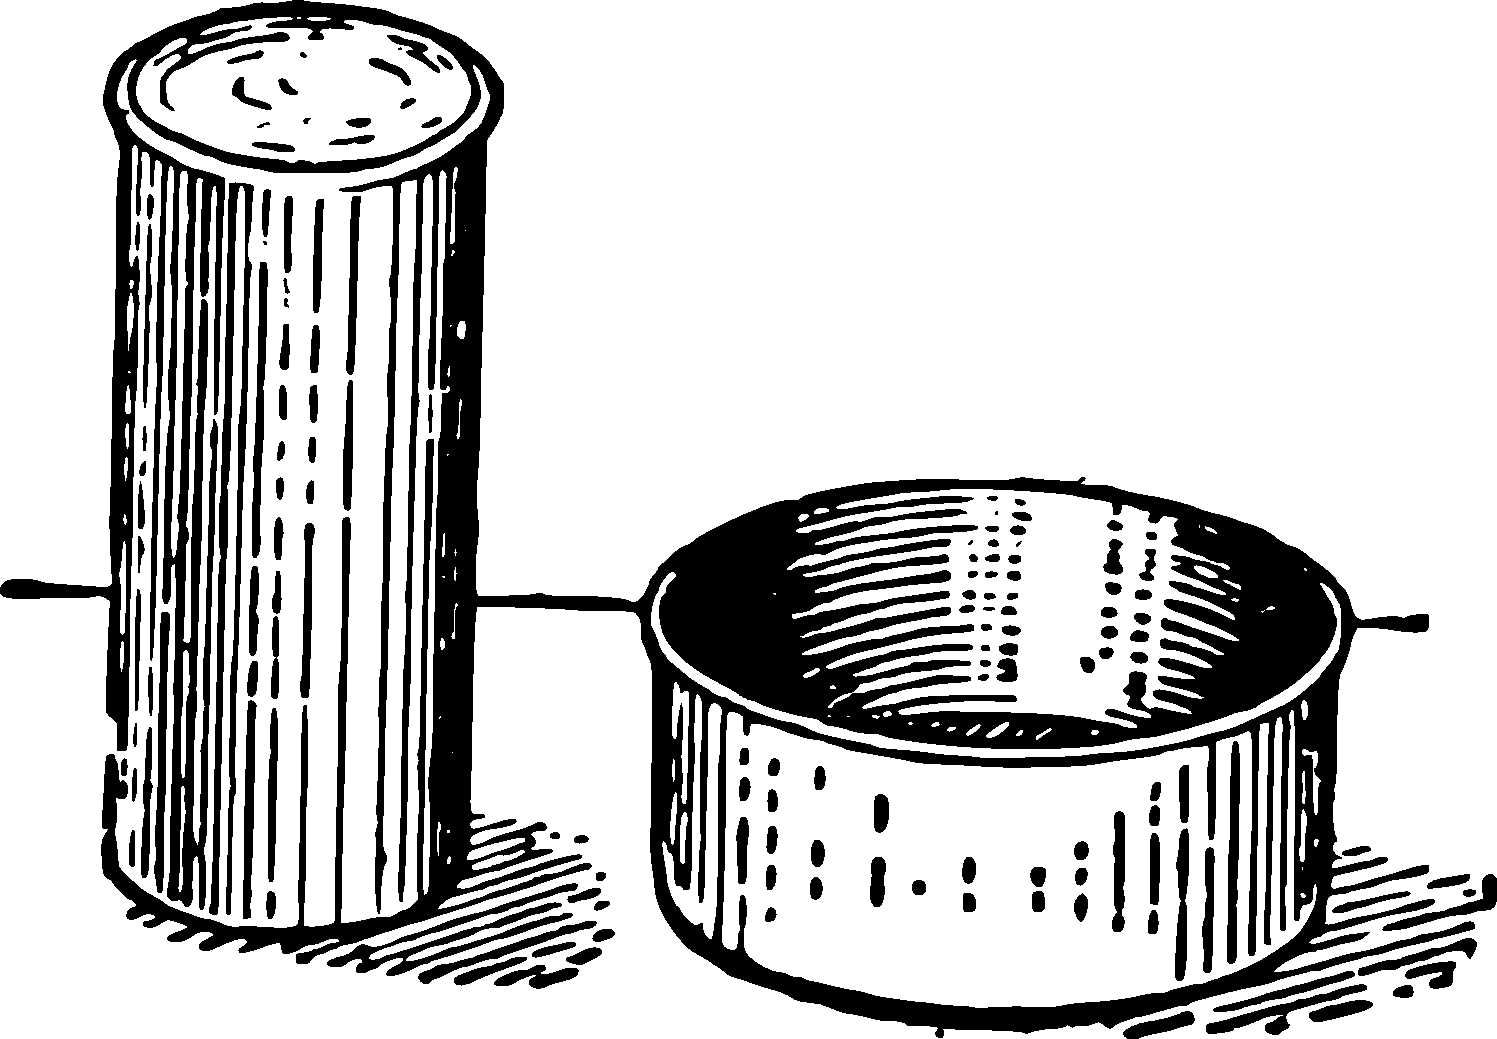
\includegraphics[width=\textwidth]{figures/ch-11/fig-165.pdf}
\sidecaption{Which jar holds more?\label{fig-165}}
\end{marginfigure}

\ques Which of the two jars (\figr{fig-165}) holds more—the right, wider one, or the left, three times taller but half as wide one?

\ans For many, it will probably be surprising that in this case, the tall jar holds less than the wide one. However, it’s easy to verify this with a calculation. The base area of the wide jar is $2 \times 2$, that is, four times greater than that of the narrow jar; its height is only three times less. Therefore, the volume of the wide jar is 4/3 times greater than the narrow one. If you pour the contents of the tall jar into the wide one, it will fill only 3/4 of it (\figr{fig-166}).


\begin{marginfigure}[-1cm]%[h!]
\centering
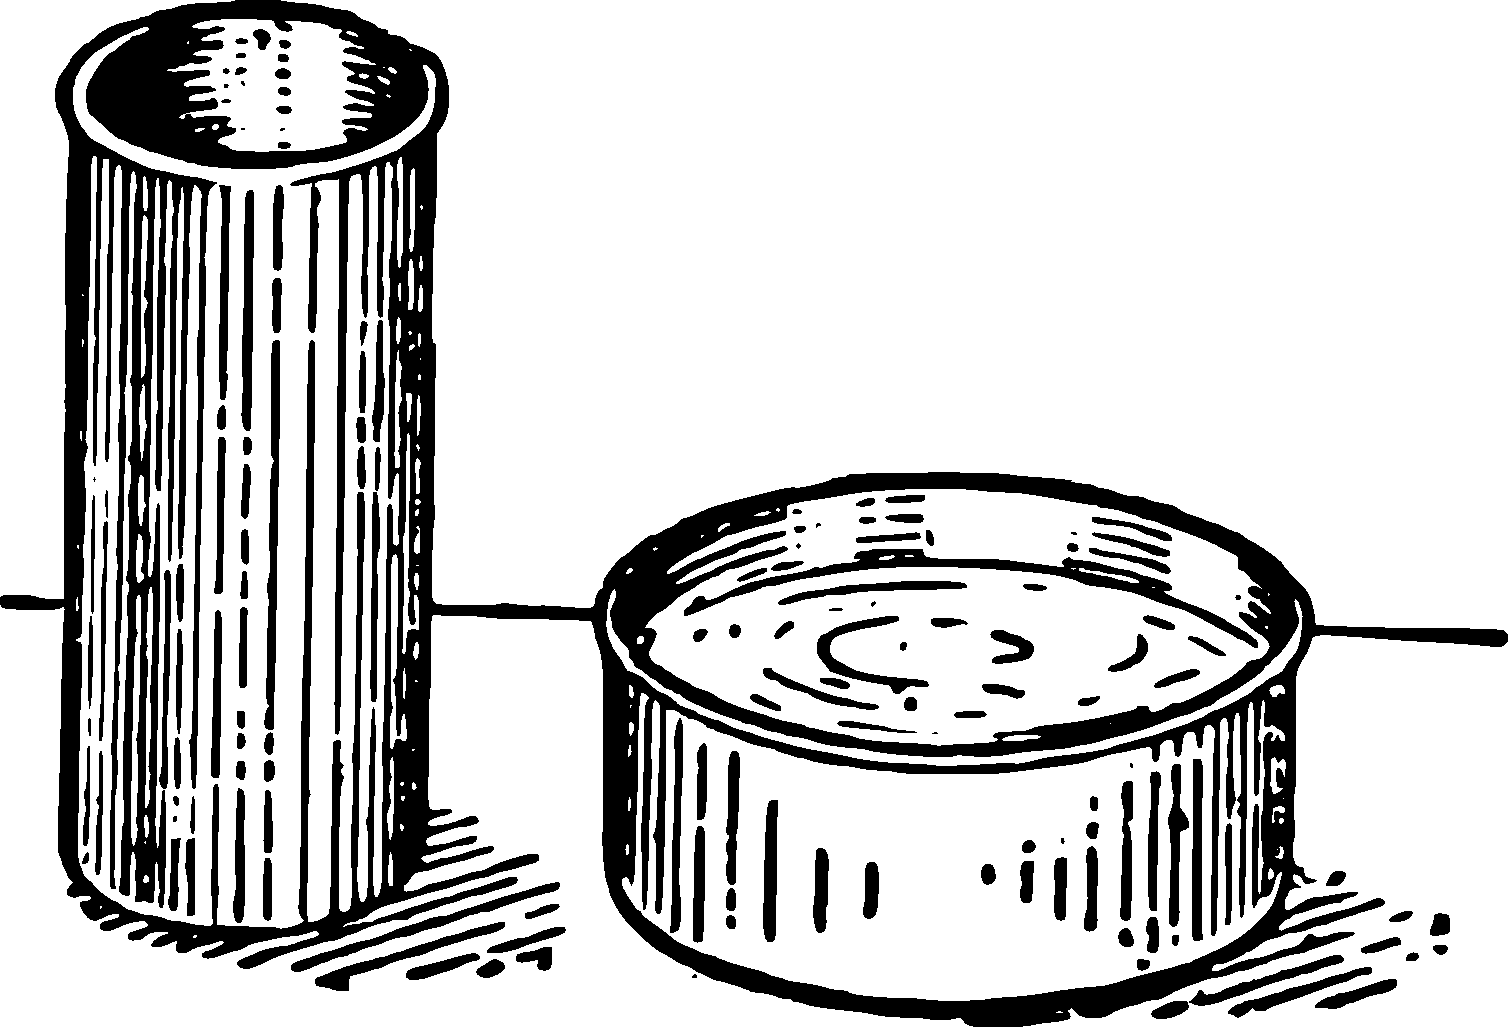
\includegraphics[width=\textwidth]{figures/ch-11/fig-166.pdf}
\sidecaption{Result of pouring the contents of the tall jar into the wide one.\label{fig-166}}
\end{marginfigure}


\section{Gigantic Cigarette}
\label{sec-11.5}


\ques In the window of a tobacco store, there is an enormous cigarette displayed, 15 times longer and 15 times thicker than a regular one. If stuffing a normal-sized cigarette requires half a gram of tobacco, how much tobacco was needed to stuff the gigantic cigarette in the window?

\ans \begin{equation*}%
\frac{1}{2} \times 15 \times 15 \times 15 = 1700 \,\, \text{gram}, 
\end{equation*}
i.e., about 1.7 kilogrammes.

\section{Ostrich Egg Task}
\label{sec-11.6}

\ques In \figr{fig-166}, a chicken egg is shown on the right and an ostrich egg on the left (the middle image is an egg of the extinct elephant bird, which will be discussed in the next problem). Look closely at the drawing and estimate how many times the volume of the ostrich egg is larger than that of the chicken egg. At first glance, it may not seem like a significant difference. The result obtained through proper geometric calculation is quite astonishing.


\begin{figure}[h!]
\centering
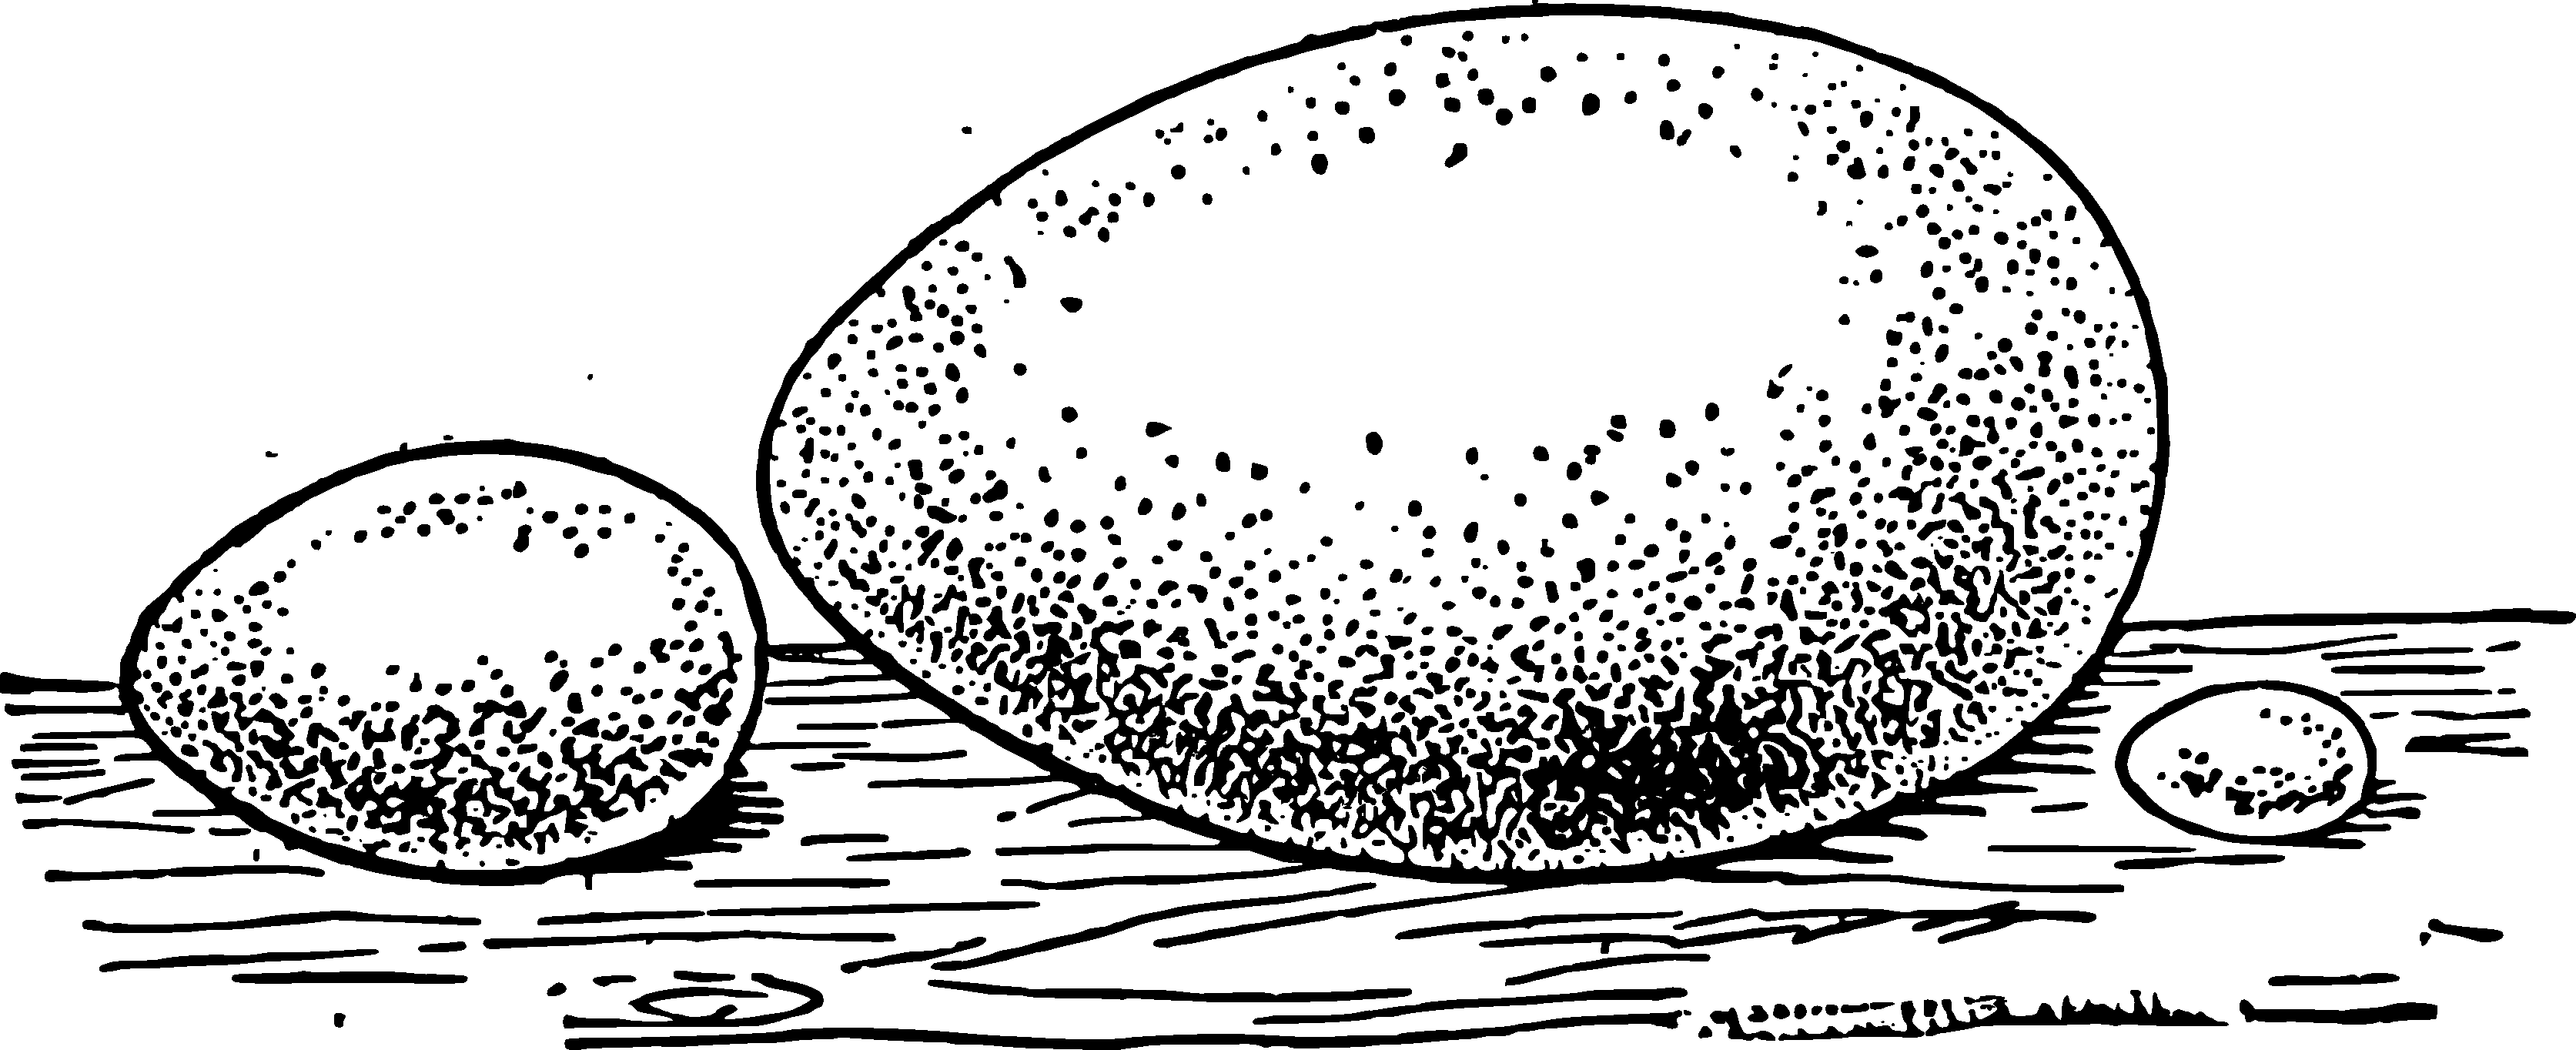
\includegraphics[width=0.9\textwidth]{figures/ch-11/fig-167.pdf}
\sidecaption{Comparative sizes of ostrich, elephant bird, and chicken eggs.\label{fig-167}}
\end{figure}

\ans By direct measurement on the drawing, we see that the ostrich egg is 2.5 times longer than the chicken egg. Consequently, the volume of the ostrich egg is greater than the volume of the chicken egg by
\begin{equation*}%
2.5 \times 2.5 \times 2.5 = 15, 
\end{equation*}
i.e., approximately 15 times.

One such egg could provide breakfast for a family of five, assuming each person is satisfied with an omelet made from three eggs.

\section{Elephant Bird Egg}
\label{sec-11.7}


\ques In Madagascar, there once lived giant ostriches known as elephant birds, which laid eggs 28 cm long (the middle figure in \figr{fig-166}). Meanwhile, a chicken egg is 5 cm long. How many chicken eggs correspond in volume to one egg of the Madagascan ostrich?


\ans By multiplying \( 28/5 \times 28/5 \times \), we get approximately 170. One elephant bird egg is equivalent to almost 200 chicken eggs! More than fifty people could be satisfied with one such egg, which, as easy to calculate, weighed 8-9 kg. (Let us remind the reader of the clever fantasy story by Herbert Wells about the elephant bird egg.)

\clearpage

\section{Eggs of Russian Birds}
\label{sec-11.8}



The most striking contrast in sizes, however, will be when we turn to our native nature and compare the eggs of the mute swan and the goldcrest, the smallest of all Russian birds. In \figr{fig-168}, the outlines of these eggs are shown in life size. What is the ratio of their volumes?

\begin{figure}[h!]
\centering
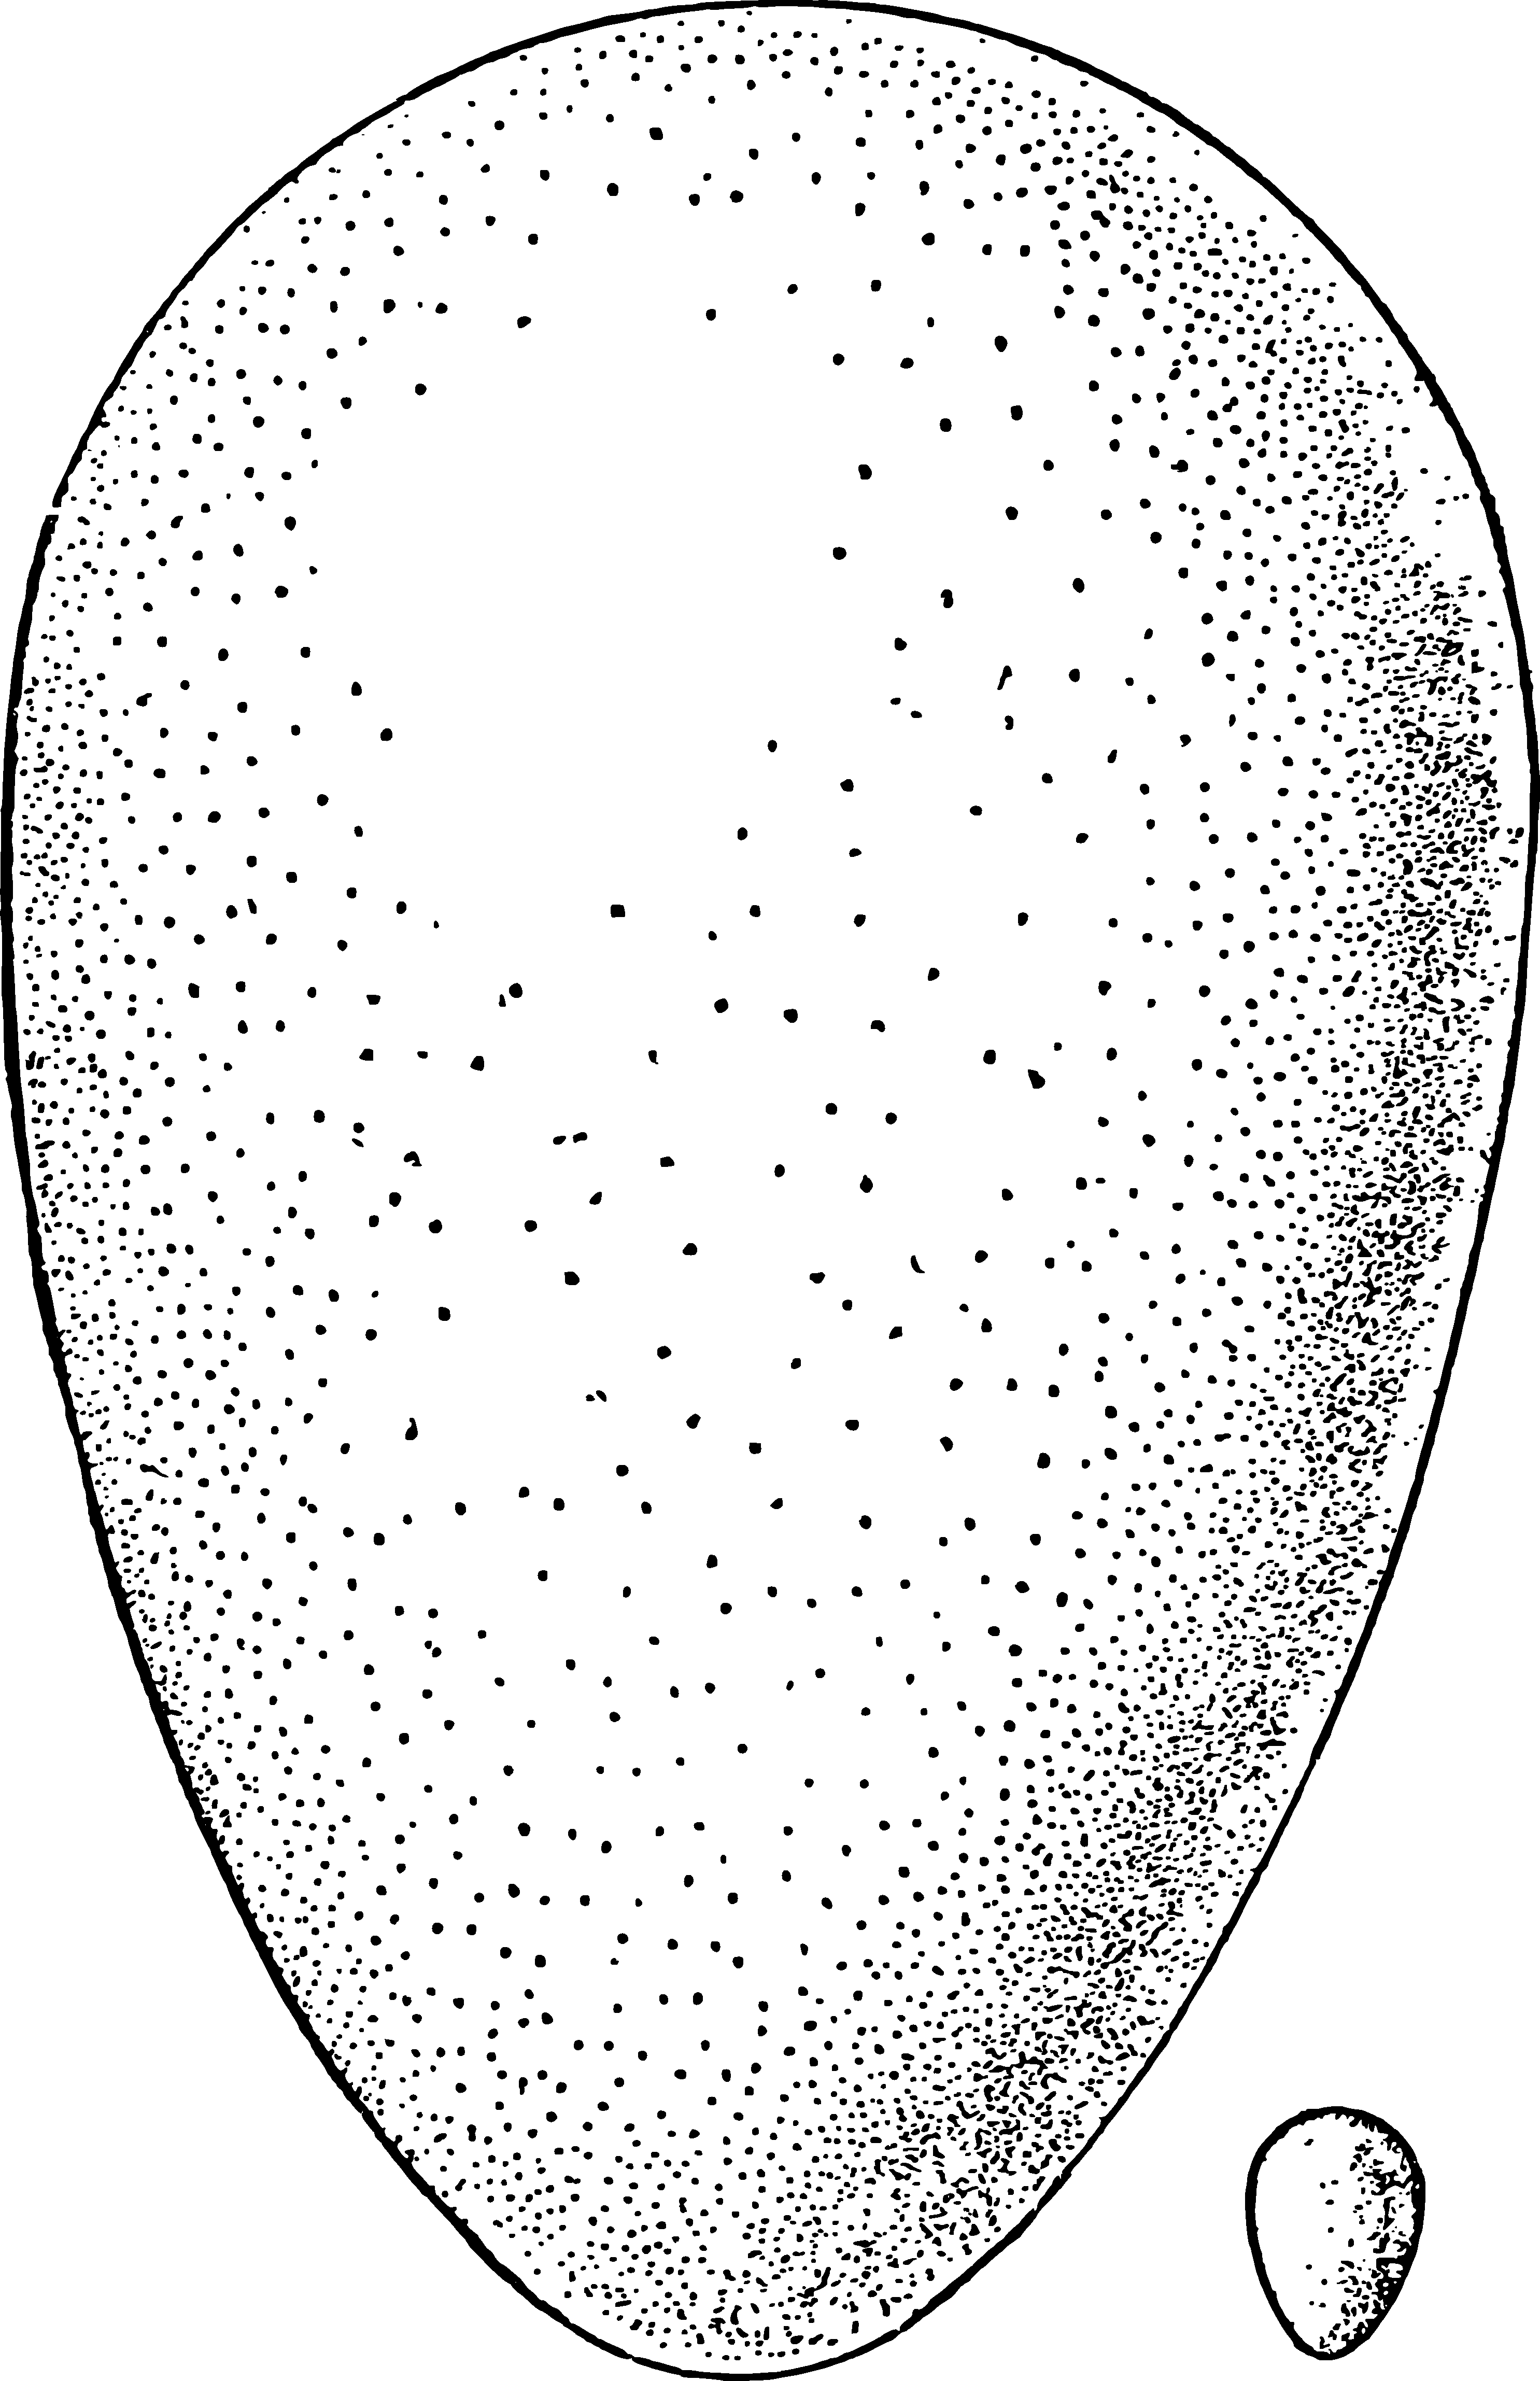
\includegraphics[width=0.7\textwidth]{figures/ch-11/fig-168.pdf}
\sidecaption{Swan's egg and goldcrest (full size). How many times is one larger than the other in volume?\label{fig-168}}
\end{figure}

\ans By measuring the length of both eggs, we get 125 mm and 13 mm. By also measuring their width, we get 80 mm and 9 mm. It is easy to see that these numbers are almost proportional; verifying the proportion
\begin{equation*}%
\frac{125}{80} \approx \frac{13}{9},
\end{equation*}
and comparing the products of the extremes and means, we have: 1125 and 1040 -- numbers that differ little. Hence, we conclude that assuming these eggs are geometrically similar bodies, we will not make a significant error. Therefore, the ratio of their volumes is approximately equal to
\begin{equation*}%
\frac{80^3}{9^3} = \frac{512000}{750} \approx 700.
\end{equation*}

Thus, the volume of a swan egg is about 700 times that of a goldcrest egg!

\section[Weight of the eggshell]{Determine the weight of the eggshell without breaking the eggs}
\label{sec-11.9}


\ques You have two eggs of the same shape but different sizes. You need to approximately determine the weight of their shells without breaking them. What measurements, weightings, and calculations are necessary to perform this task? The thickness of the shells can be considered identical for both eggs.



\ans Measure the length of the major axis of each egg: let these be \( D \) and \( d \). Let the weight of the shell of the first egg be \( x \), and the second egg be \( y \). The weight of the shell is proportional to its surface area, which is proportional to the square of its linear dimensions. Therefore, assuming the shell thickness of both eggs is the same, we set up the proportion:
\begin{equation*}%
\frac{x}{y} = \frac{D^2}{d^2}.
\end{equation*}
\textbf{Weigh the eggs:} let these weights be \( P \) and \( p \). The weight of the egg's content can be considered proportional to its volume, i.e., the cube of its linear dimensions:
\begin{equation*}%
\frac{(P - x)}{(p - y)} = \frac{D^3}{d^3}.
\end{equation*}
We have a system of two equations with two unknowns; solving it, we find:
\begin{equation*}%
x = \frac{p \cdot D^3 - P \cdot d^3}{d^2 \cdot (D - d)}; \quad
y = \frac{p \cdot D^3 - P \cdot d^3}{D^2 (D - d)}.
\end{equation*}


\section{The sizes of our coins}
\label{sec-11.10}

The weight of our coins is proportional to their value, i.e. a two—kopeck coin weighs twice as much as a kopeck coin, a three-kopeck coin weighs three times more, etc. The same is true for silver in exchange; a two-kopeck piece, for example, is twice as heavy as a dime. And since homogeneous coins usually have a geometrically similar shape, knowing the diameter of one change coin, you can calculate the dimensions of others that are homogeneous with it. Here are examples of such calculations.

\ques The diameter of a five-kopeck coin is 25 mm. What is the diameter of a three-kopeck coin?

\ans The weight, and therefore the volume, of a three-kopeck coin is 3/5, i.e., 0.6 of the volume of a five-kopeck coin. Therefore, its linear dimensions should be $\sqrt[3]{0.6}$ times smaller, i.e., 0.84 the size of a five-kopeck coin. Hence, the required diameter of the three-kopeck coin should be $0.84 \times 25$, i.e., 21 mm (actually 22 mm).


\section{Coin worth a million roubles}
\label{sec-11.11}


\ques Imagine a fantastic silver coin worth a million roubles, which has the same shape as a 2-kopek coin, but correspondingly heavier. What would be the approximate diameter of such a coin? If it were placed on its edge next to a car, how many times taller would it be than the car?



\ans The dimensions of the coin would not be as enormous as one might think. Its diameter would be only about 3.8 m -- just above one floor. Indeed, since its volume is larger than that of the two-kopek coin by 5,000,000 times, its diameter (as well as thickness) would be larger by $\sqrt[3]{5000000}$, i.e., only 172 times.

Multiplying 22 mm by 172, we get approximately 3.8 m -- unexpectedly modest dimensions for a coin of such value.

\begin{figure}[h!]
\centering
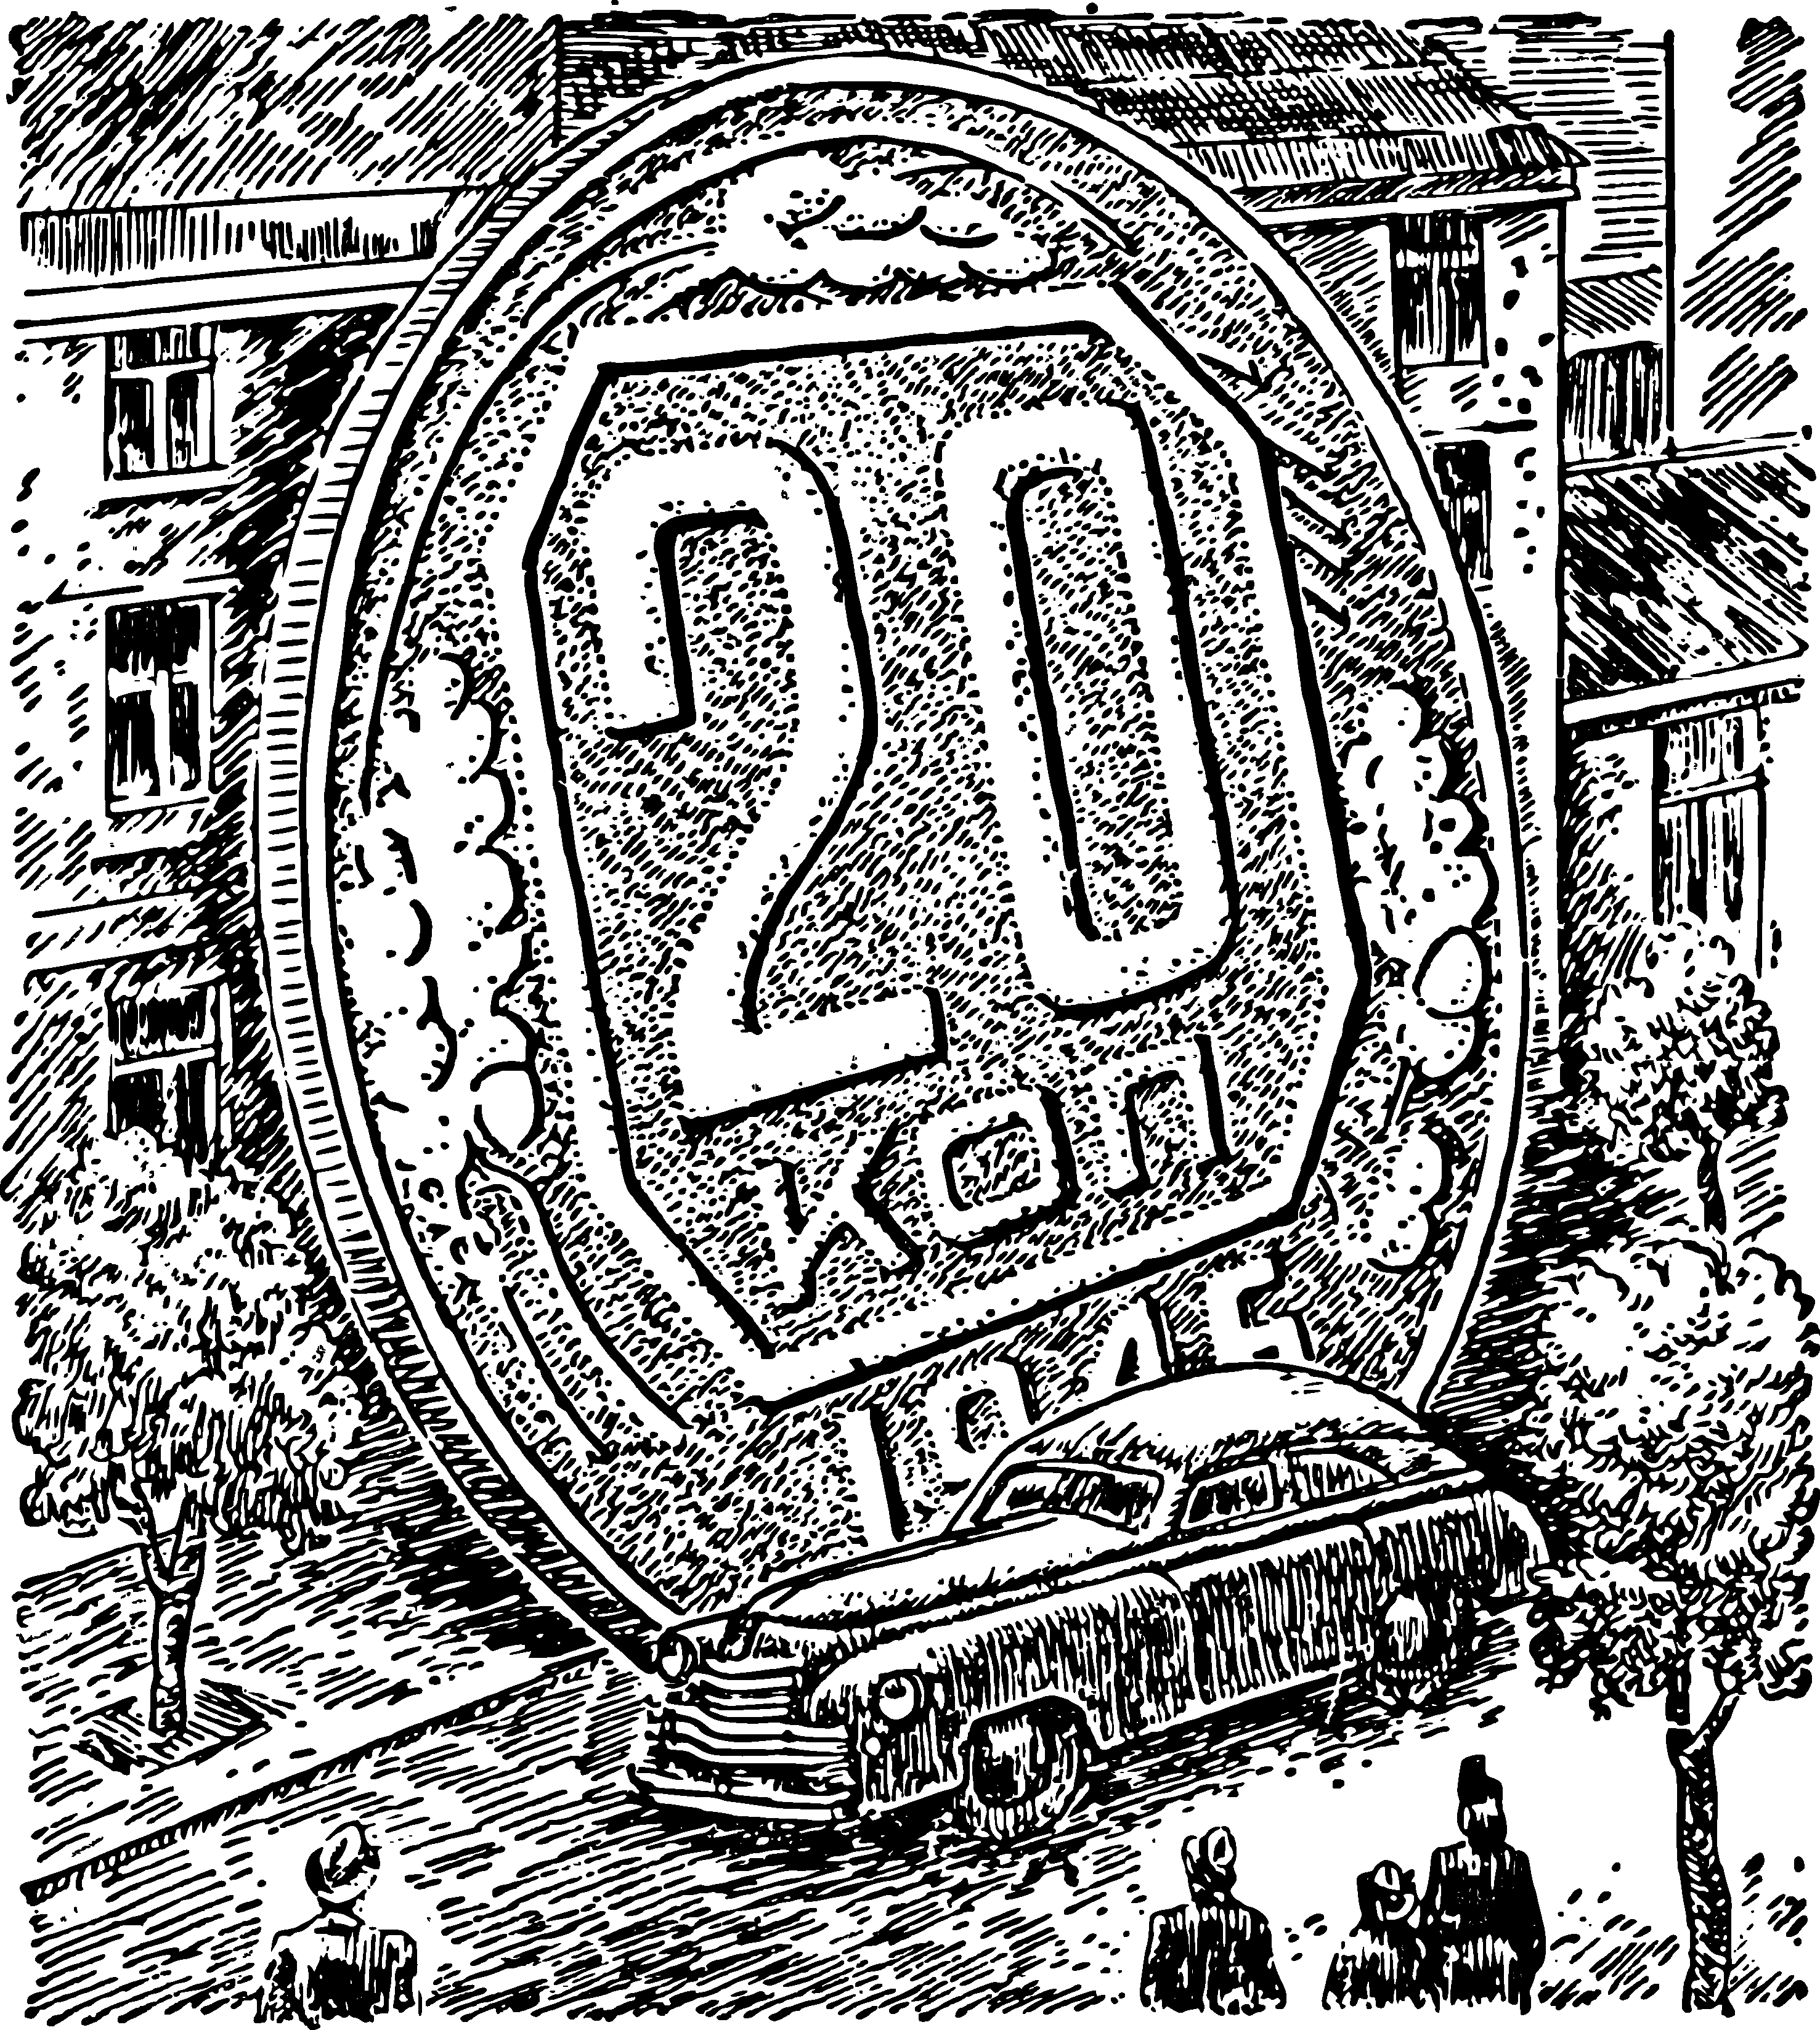
\includegraphics[width=0.7\textwidth]{figures/ch-11/fig-169.pdf}
\sidecaption{What coin is equivalent to this giant two-kopeck piece?\label{fig-169}}
\end{figure}

\ques Calculate which coin would be equivalent to a two-hryvnia coin enlarged to the size of a four-story building (in height) (\figr{fig-169}.

\section{Visual Representations}
\label{sec-11.12}



The reader who has acquired the skill of comparing volumes of geometrically similar bodies based on their linear dimensions from the previous examples will no longer be caught off guard by questions of this kind. Therefore, they can easily avoid the mistakes of some seemingly vivid images that often appear in illustrated magazines.


\ques Here is an example of such images. If a person consumes an average of 400 grams of meat per day, then over 60 years of life, this would amount to about 9 tons. And since the weight of a bull is about 0.5 ton, a person could claim to have consumed 18 bulls by the end of their life.

In the accompanying \figr{fig-170}, reproduced from an English magazine, this gigantic bull is depicted next to a person consuming it over a lifetime. Is the picture accurate? What would be the correct scale?

\begin{figure}[h!]
\centering
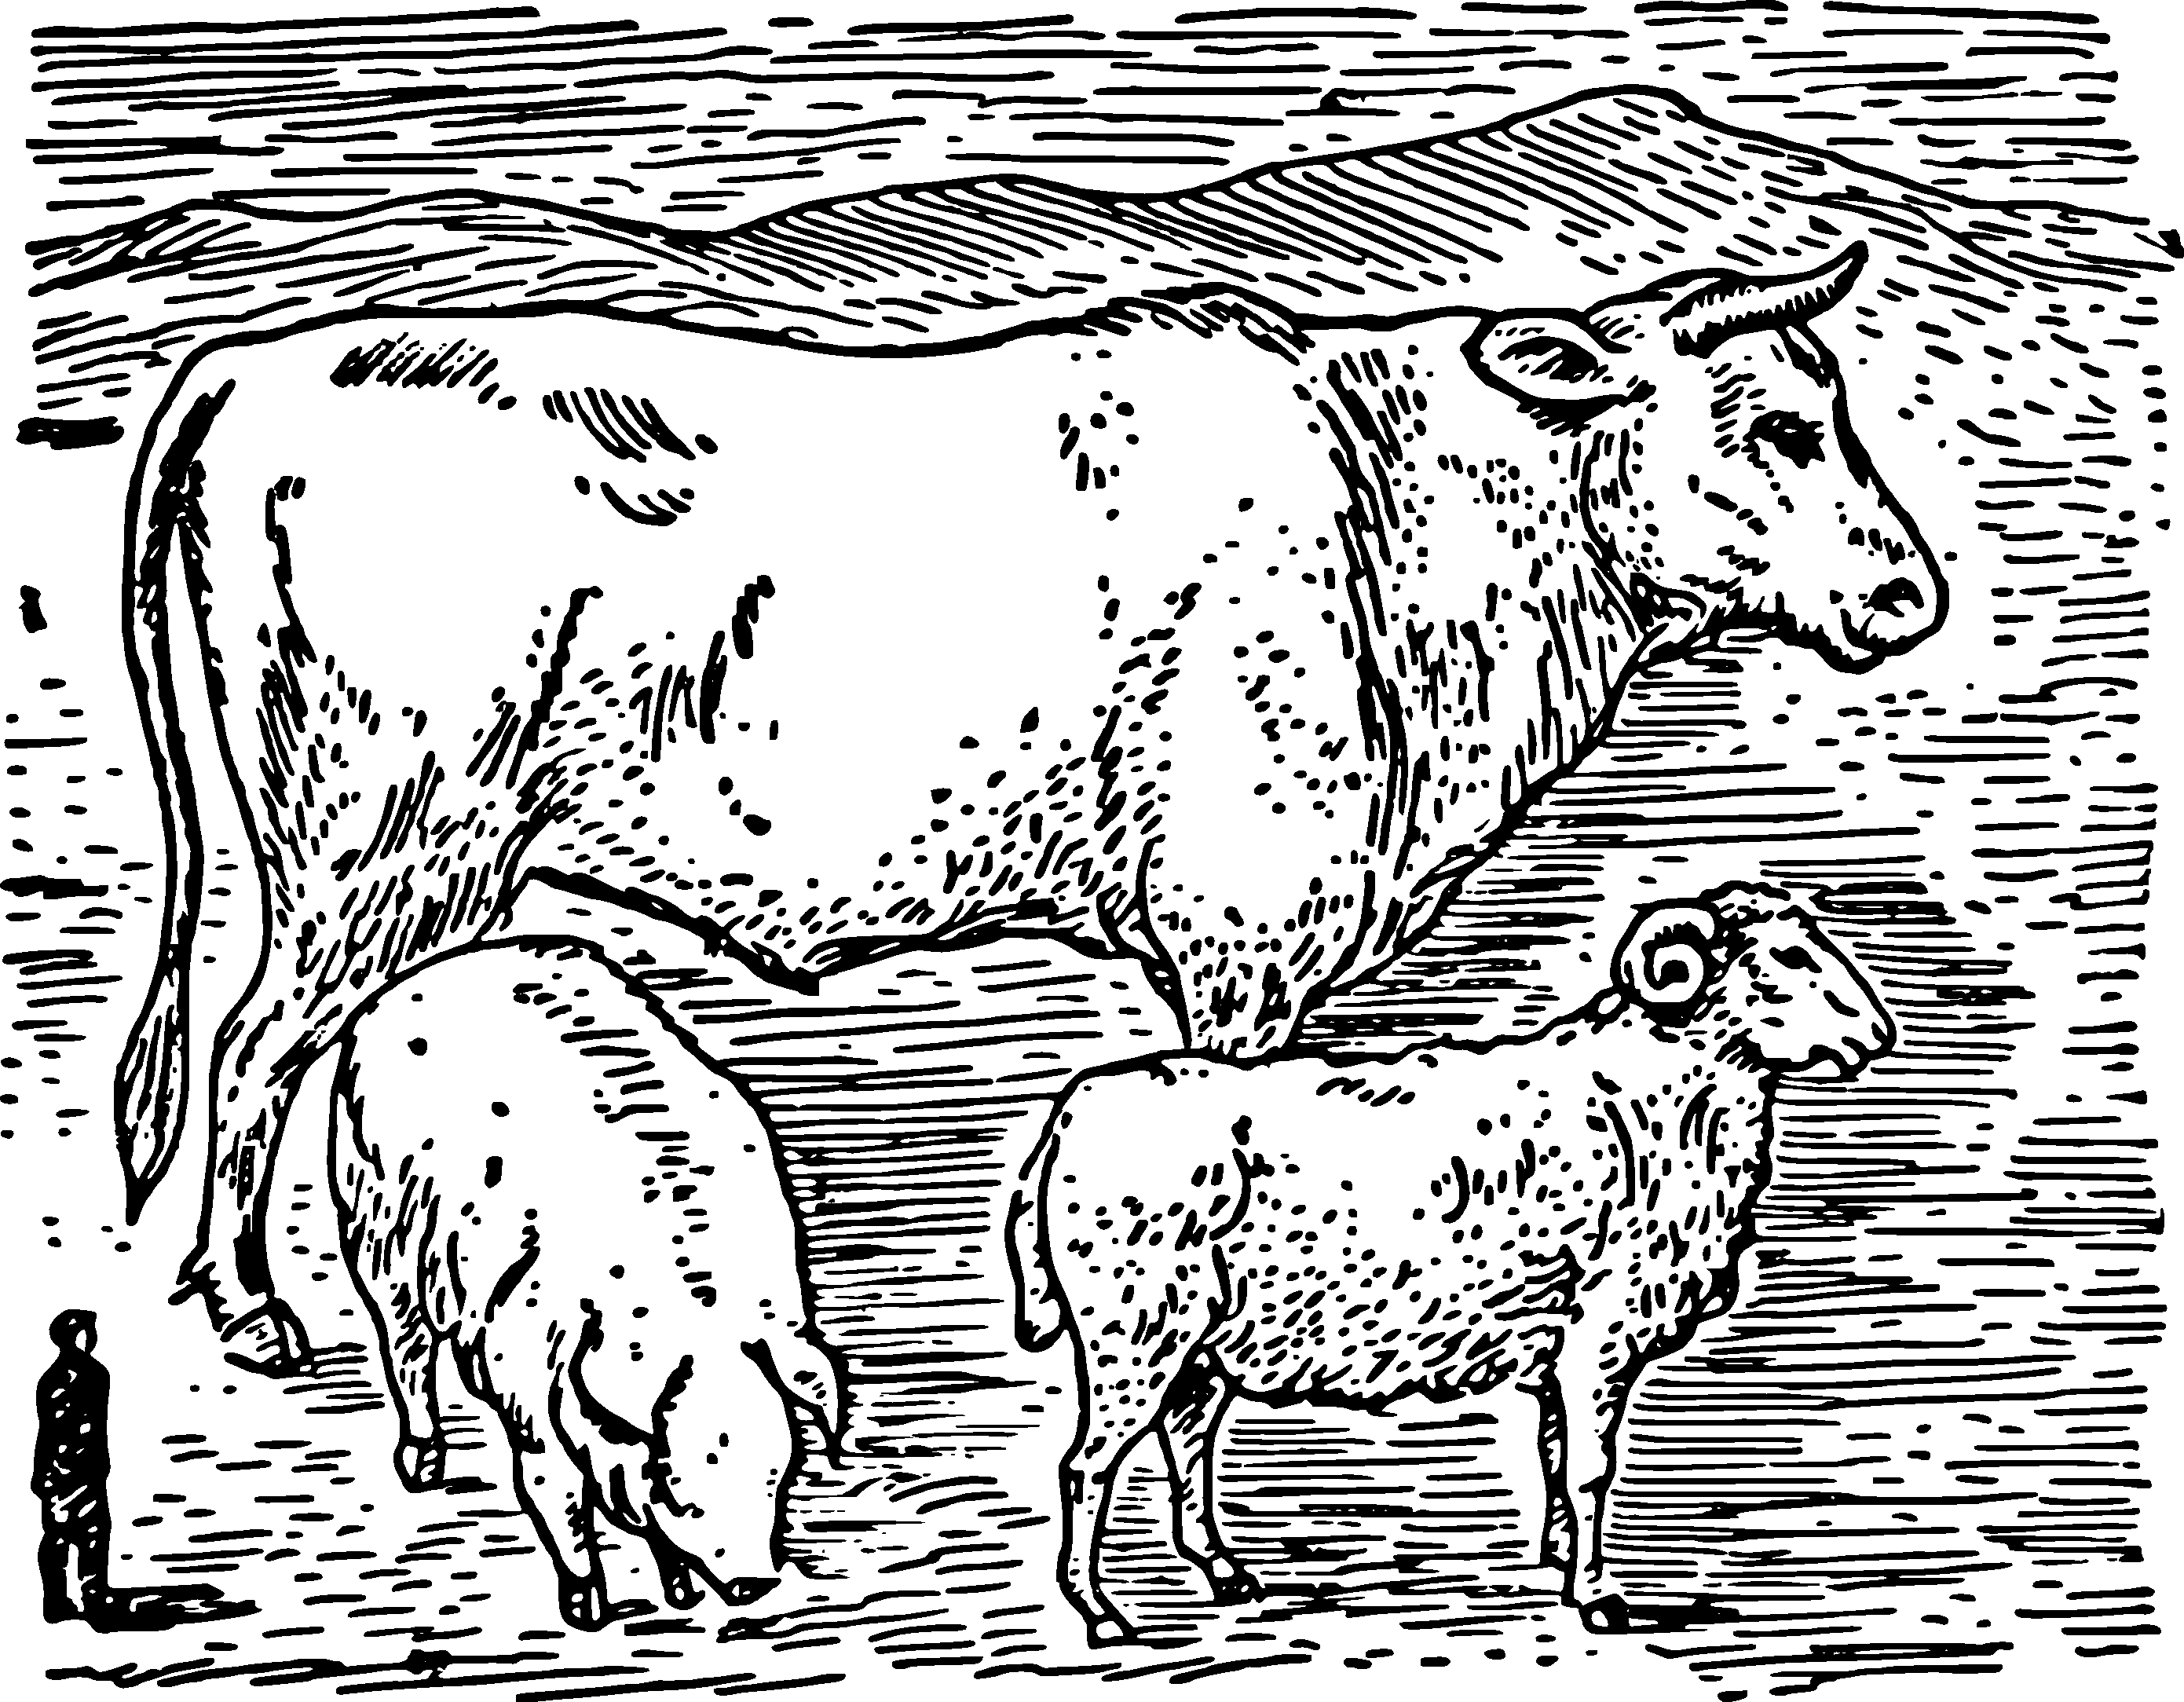
\includegraphics[width=0.8\textwidth]{figures/ch-11/fig-170.pdf}
\sidecaption{How much meat a person eats during their lifetime (to detect an error in the image).\label{fig-170}}
\end{figure}


\ans The picture is inaccurate. The bull depicted here is 18 times taller than normal and, of course, 18 times longer and thicker as well. Therefore, in terms of volume, it is $18 \times 18 \times 18 = 5832$ times larger than a normal bull. For a person to consume such a bull, they would have to live for at least two thousand years!

The correctly depicted bull should be taller, longer, and thicker than the normal one by only $\sqrt[3]{18}$, or 2.6 times; this would not be as impressive in the picture, so it wouldn't serve as a striking illustration of the amount of meat consumed by humans.



\begin{figure}[h!]
\centering
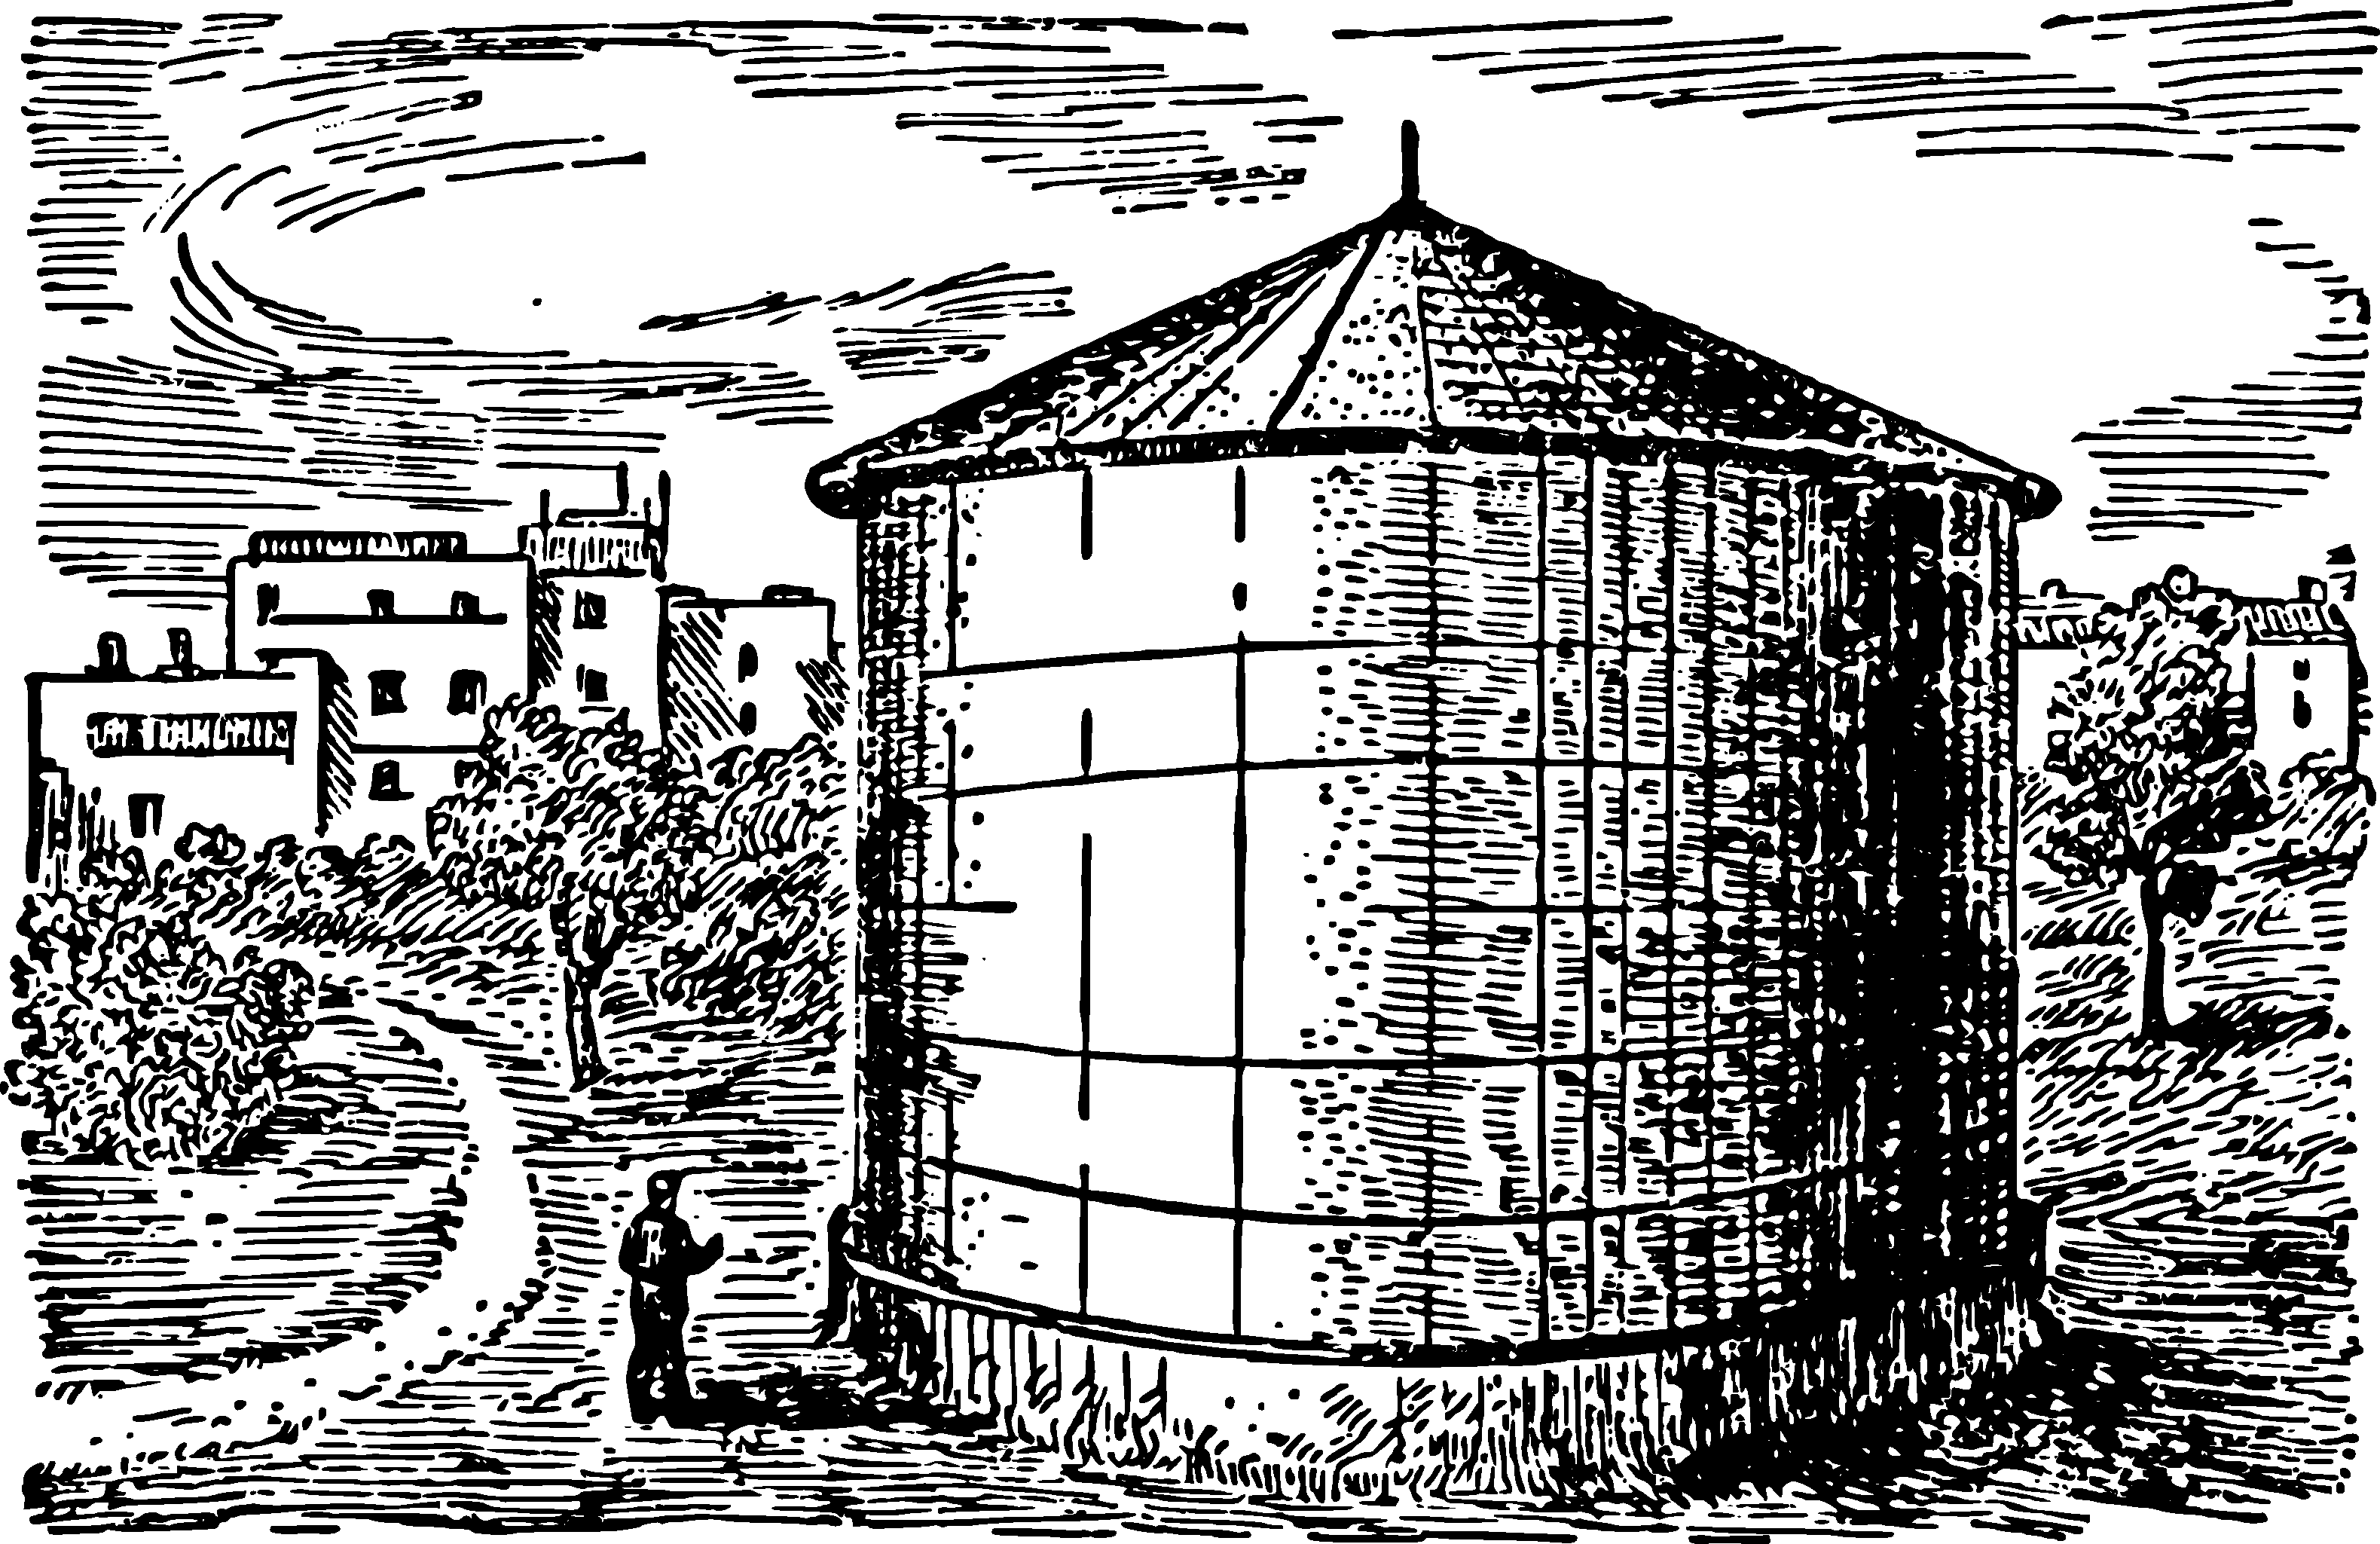
\includegraphics[width=0.9\textwidth]{figures/ch-11/fig-171.pdf}
\sidecaption{How much water does a person drink over a lifetime (what mistake did the artist make?).\label{fig-171}}
\end{figure}


\ques In \figr{fig-171}, another illustration from the same field is reproduced. A person consumes 1.5 litres of various liquids per day (7-8 glasses). Over 70 years of life, this amounts to about 40,000 litres. Since a bucket holds 12 litres, the artist needed to depict some vessel that is 3300 times larger than a bucket. He thought he had done this in \figr{fig-171}. Is he correct?


\ans In the picture, the dimensions of the tank are greatly exaggerated. The vessel should be taller and wider than a normal bucket by only $\sqrt[3]{3300} = 14.9$, rounded to 15 times. If the height and width of a normal bucket are 30 cm, then to accommodate all the water we drink in our lifetime, a bucket with a height of 4.5 meters and the same width would suffice. \figr{fig-172} depicts this vessel in the correct scale.


\begin{figure}[h!]
\centering
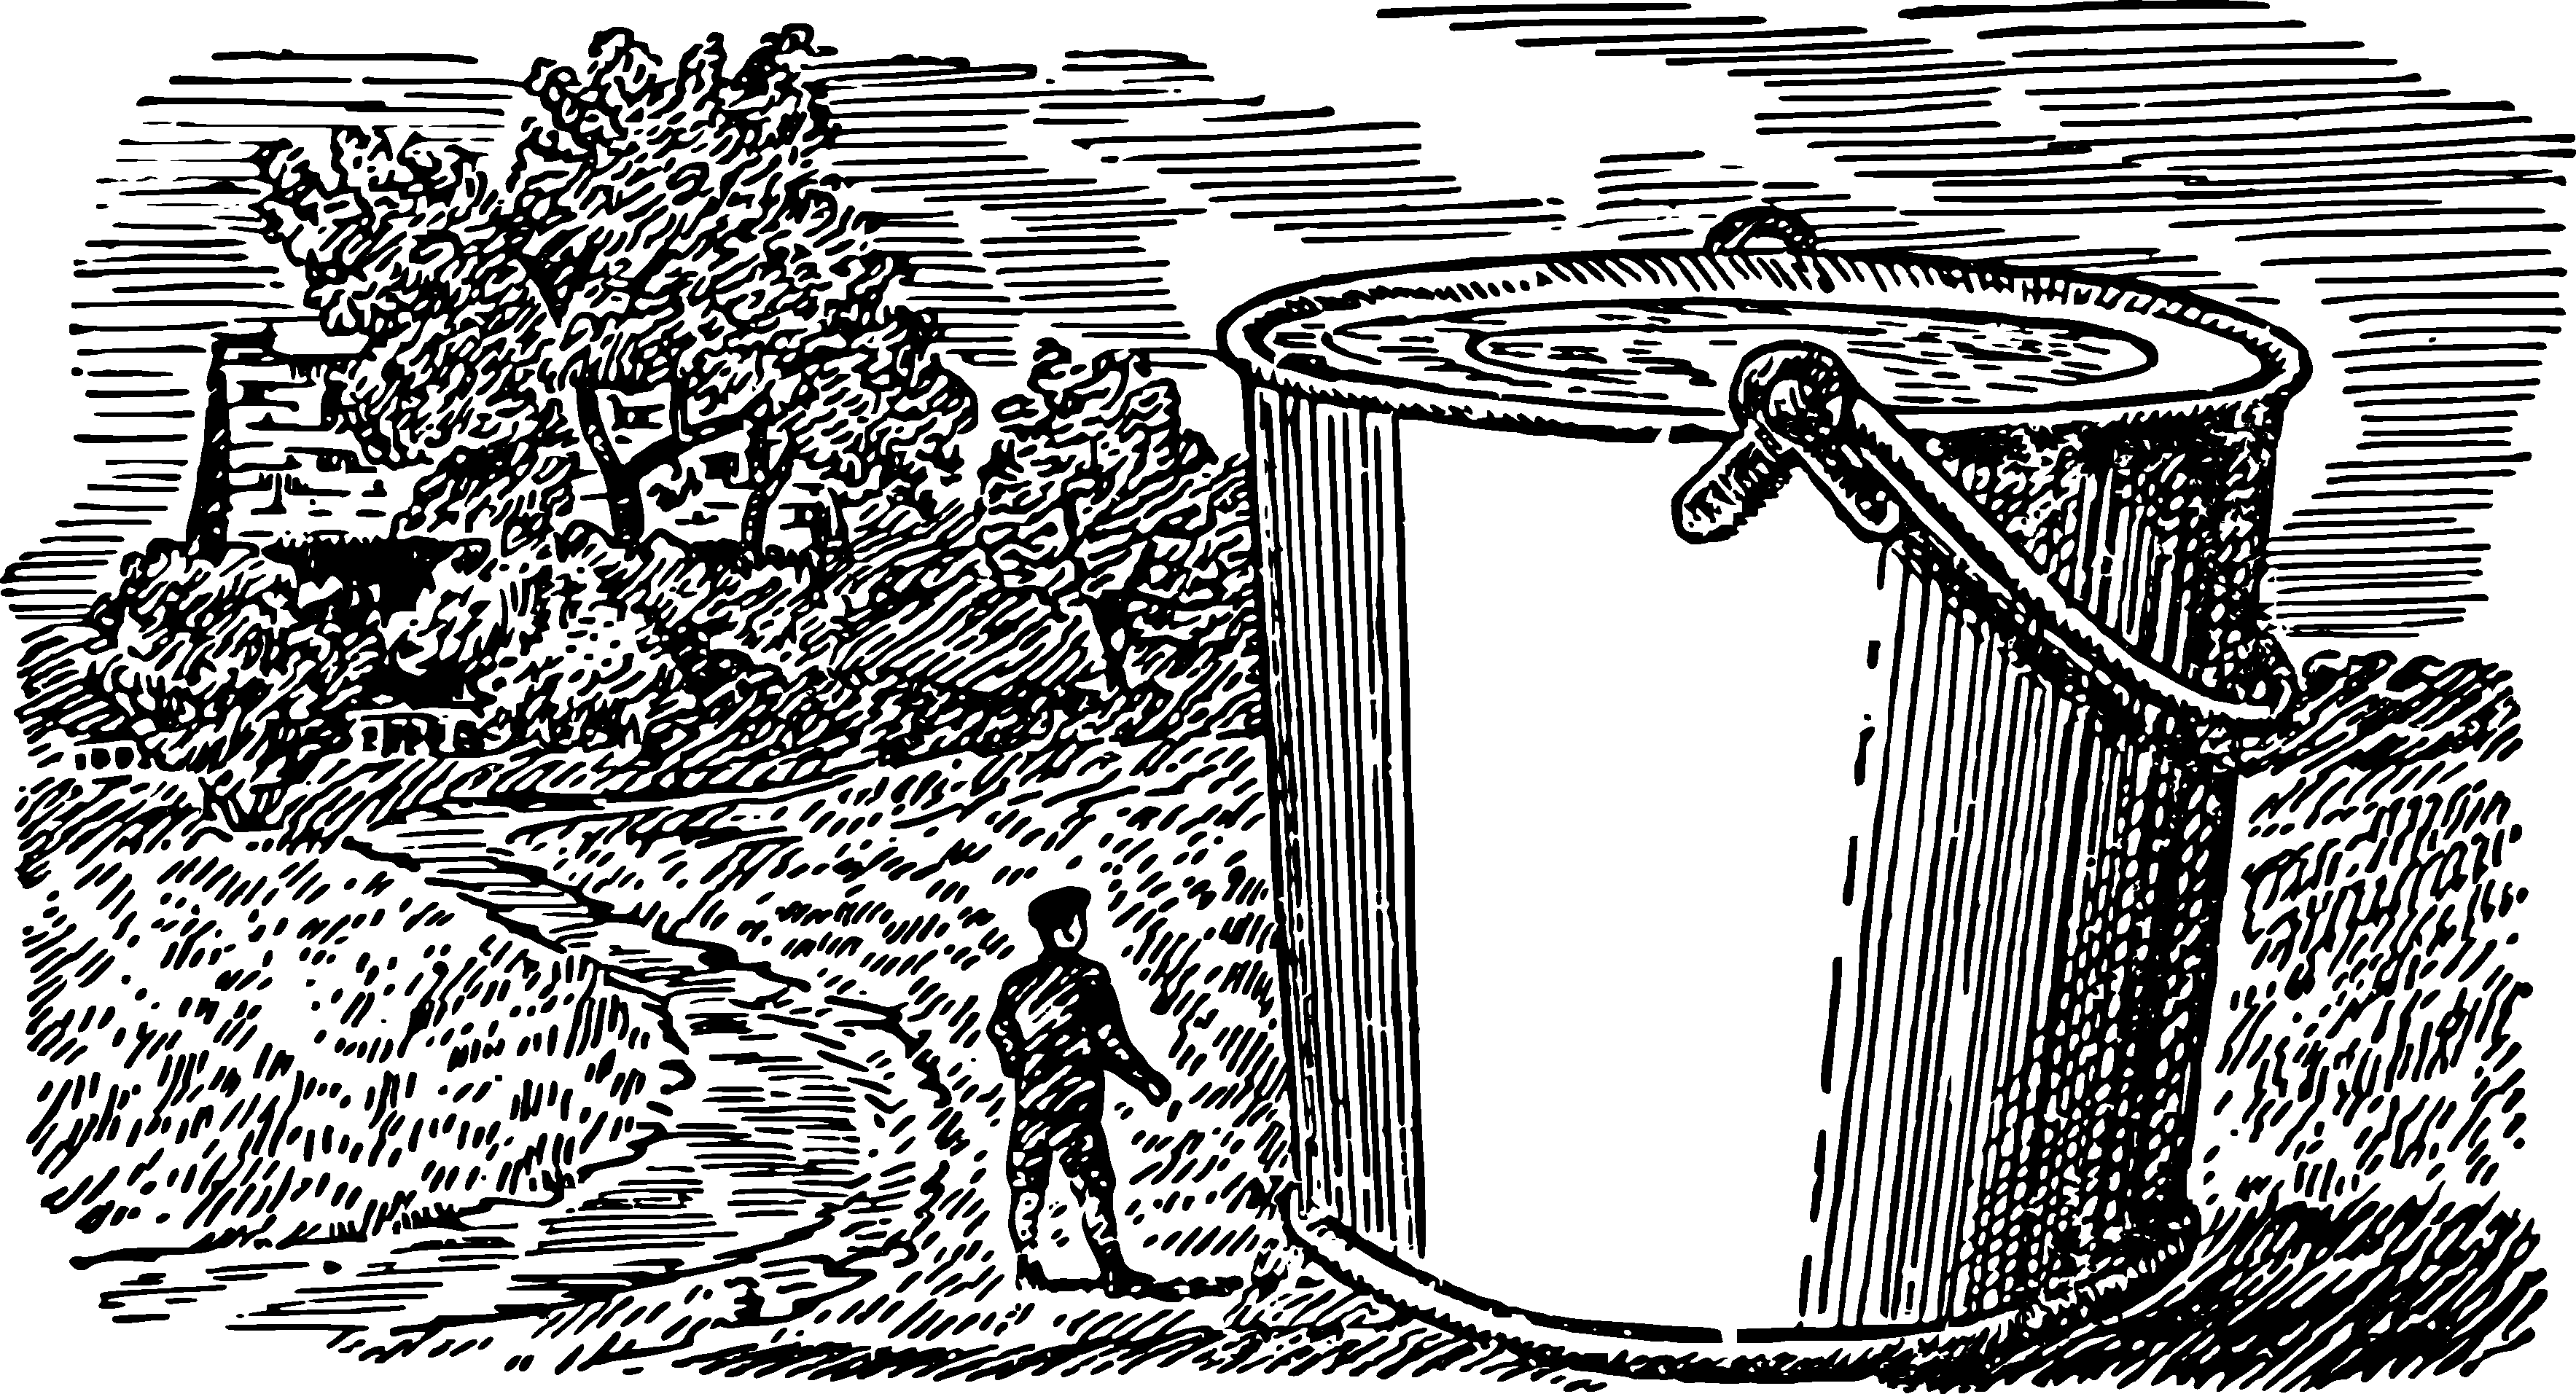
\includegraphics[width=0.9\textwidth]{figures/ch-11/fig-172.pdf}
\sidecaption{The same (see \figr{fig-171}) - correct depiction.\label{fig-172}}
\end{figure}

The examples considered show, among other things, that representing statistical numbers in the form of volumetric bodies is not sufficiently illustrative and does not produce the impression usually expected. Bar charts have an undeniable advantage in this regard.

\section{Our Normal Weight}
\label{sec-11.13}

If we assume that all human bodies are geometrically similar (which is only true on average), then we can calculate people's weight based on their height (the average height of a person is 1.75 meters, and the average weight is 65 kg). The results obtained from such ``calculations'' may be surprising to many.

Let's assume you are shorter than average by 10 cm. What weight is considered normal for you?

Often, in everyday life, this problem is solved by subtracting from the normal weight the percentage that corresponds to 10 cm from the average height. In this case, for example, subtracting 65 kg by 10/175, the resulting weight -- 62 kg -- is considered normal.

This is an incorrect calculation.

The correct result can be obtained by calculating it from the proportion:
\begin{align*}%
\frac{65}{x} & = \frac{1.75^{3}}{1.65^{3}}, \,\, \text{from which}\\
 x & \approx \SI{54}{\kilo\gram}.
\end{align*}
The difference from the usually obtained result is quite significant -- 8 kg.

Conversely, for a person whose height is 10 cm above average, the normal weight is calculated from the proportion:
\begin{equation*}%
\frac{65}{x} = \frac{1.75^{3}}{1.85^{3}},
\end{equation*}
From this, \( x = 78 \) kg, which is 13 kg more than average. This increase is much more significant than commonly thought.

Undoubtedly, such correctly performed calculations should have significant importance in medical practise for determining normal weight, calculating medication dosage, and so on.

What then should be the relationship between the weight of a giant and a dwarf? To many, I'm sure, it would seem improbable that a giant could be 50 times heavier than a dwarf. However, correct geometric calculations lead to this.

One of the tallest giants, whose existence is well documented, was the Austrian Winkelmeier at a height of 278 cm; another, from Alsace, Krau, was 275 cm tall; the third, an Englishman named O'Brick, was reported to have reached 268 cm. All of them were a whole meter taller than a person of normal height. In contrast, dwarfs reach about 75 cm in adulthood -- a meter shorter than normal height. What then is the ratio of the volume and weight of a giant to the volume and weight of a dwarf? It is equal to
\begin{equation*}%
\frac{275^{3}}{75^{3}}, \qor \frac{11^{3}}{3^{3}} = 49.
\end{equation*}
So, a giant is nearly fifty times heavier than a dwarf!

And if we believe the report about the Arab dwarf Agiba, who was 38 cm tall, then this ratio becomes even more striking: the tallest giant is seven times taller than this dwarf and, therefore, 343 times heavier. More reliably, Buffon's report measures a dwarf at 43 cm tall: this dwarf is 260 times lighter than the giant.

\section{Gulliver's Geometry}
\label{sec-11.14}

The author of \emph{Gulliver's Travels} carefully avoided the danger of getting lost in geometric relationships. The reader undoubtedly remembers that in the land of Lilliputians, our foot corresponded to an inch, while in the land of giants, conversely, an inch corresponded to a foot. In other words, in Lilliput, everything—people, things, and natural phenomena—were twelve times smaller than normal, while in the land of giants, they were twelve times larger. These seemingly simple relationships, however, became significantly more complicated when it came to solving questions like the following:
\begin{enumerate}
\item By how many times did Gulliver eat more for lunch than a Lilliputian?
\item By how many times did Gulliver need more fabric for a suit than the Lilliputians?
\item How much did an apple from the land of giants weigh?
\end{enumerate}
The author of \emph{Gulliver's Travels} managed these tasks quite successfully in most cases. He correctly calculated that since a Lilliputian was twelve times smaller in height than Gulliver, the volume of his body was smaller by $12 \times 12 \times 12 = 1728$ times; therefore, to satisfy Gulliver's body, 1728 times more food was needed than for a Lilliputian. And we read in \emph{Gulliver's Travels} the following description of Gulliver's lunch:
\begin{quote}
Three hundred cooks prepared meals for me. Around my house, sheds were set up where the cooking took place, and the cooks lived there with their families. When lunchtime came, I would pick up twenty servants and place them on the table, while a hundred served from the floor: some served the food, and others brought barrels of wine and other drinks on poles, carried from shoulder to shoulder. Those standing on top, as needed, lifted all this onto the table using ropes and pulleys \dots{}
\end{quote}


\begin{figure}[h!]
\centering
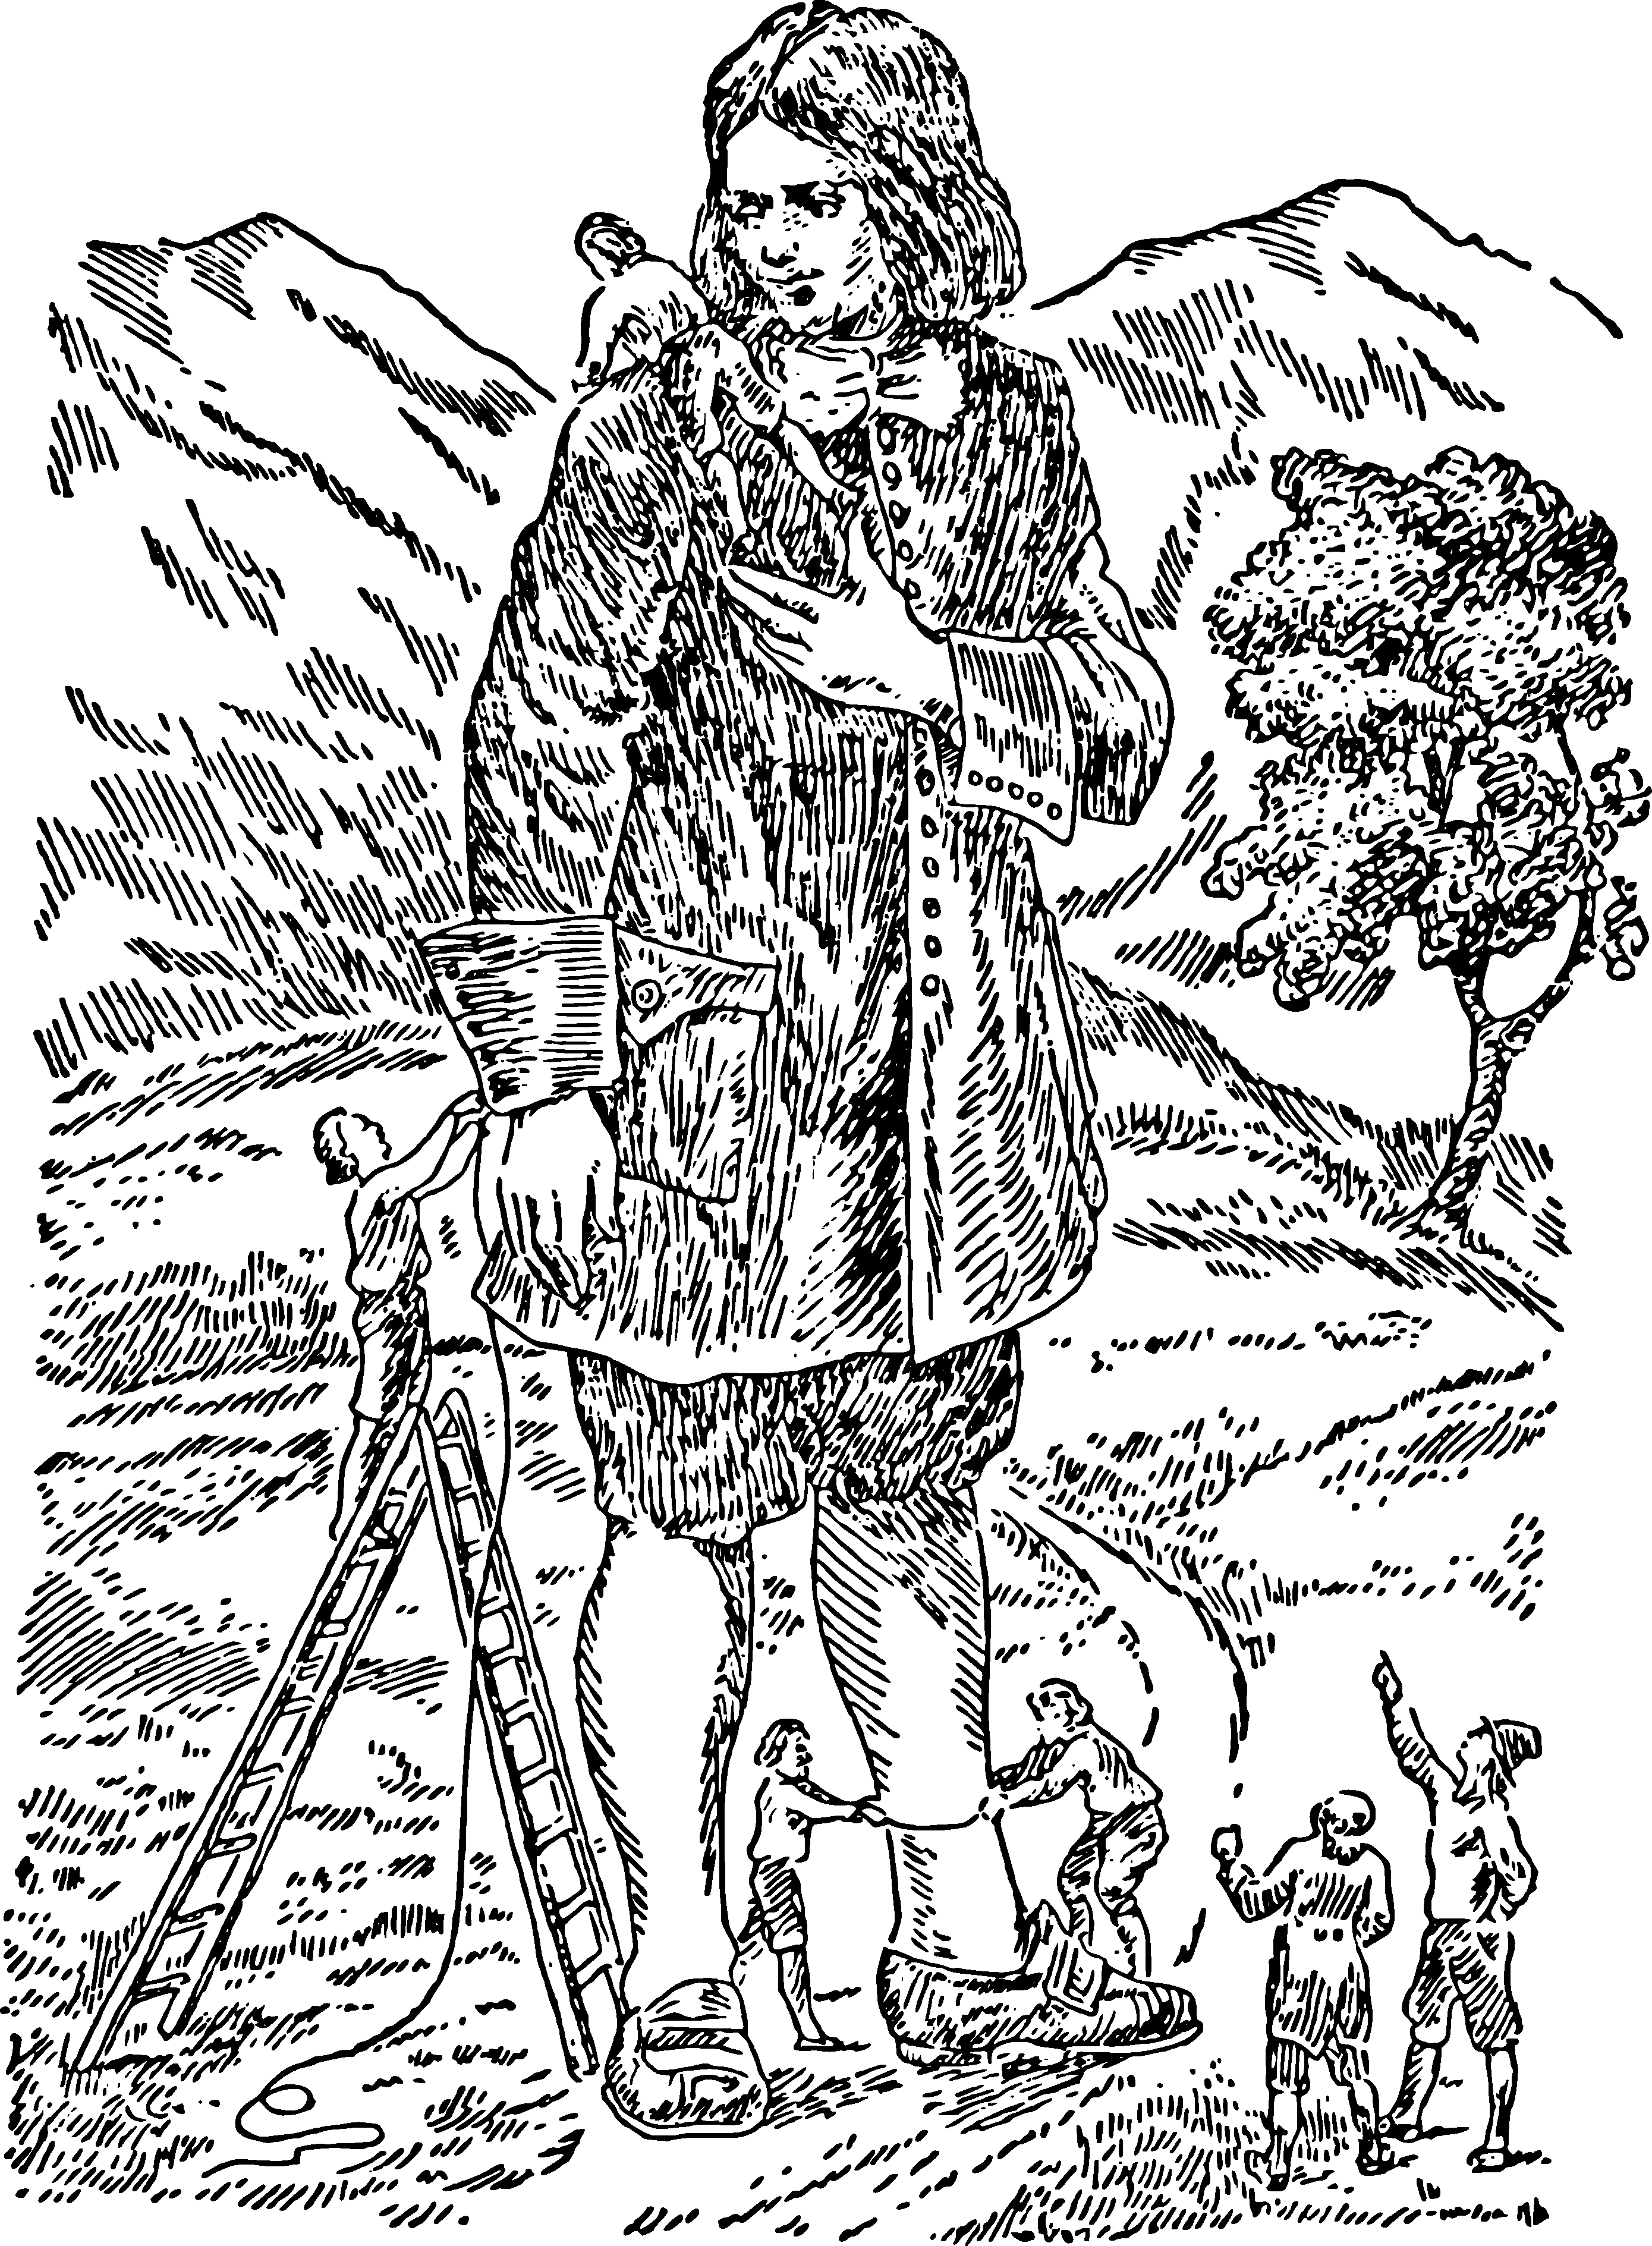
\includegraphics[width=0.7\textwidth]{figures/ch-11/fig-173.pdf}
\sidecaption{Midget tailors take measurements from Gulliver.\label{fig-173}}
\end{figure}


Swift correctly calculated the amount of material for Gulliver's suit. The surface area of his body is greater than that of the Lilliputians, by $12 \times 12 = 144$ times; he therefore needs that much more material, tailors, and so on. All of this is accounted for by Swift, who narrates on behalf of Gulliver, mentioning that ``three hundred Lilliputian tailors (see \figr{fig-173}) were assigned to me, with instructions to make a complete suit of clothes according to local standards.'' (The urgency of the task required double the number of tailors.)

The need to make such calculations arose for Swift on almost every page. And generally speaking, he executed them correctly. If, as one critic claims, Pushkin's \emph{Eugene Onegin} has ``time calculated by the calendar,'' then in Swift's \emph{Travels}, all dimensions are consistent with the rules of geometry. Only occasionally was the proper scale not maintained, especially in describing the land of the giants. Errors are sometimes encountered here.

Gulliver recounts,
\begin{quote}
Once, a court dwarf accompanied us into the garden. Seizing a convenient moment when I found myself walking under one of the trees, he grabbed a branch and shook it over my head. A hail of apples, each the size of a good-sized barrel, rained down noisily to the ground; one struck me in the back and knocked me off my feet \dots{}
\end{quote}

Gulliver managed to get up after this blow. However, it is easy to calculate that the impact from the fall of such an apple should have been truly crushing: after all, the apple is 1728 times heavier than ours, i.e., weighs 80 kg, and fell from a height twelve times greater. The energy of the impact should have exceeded the energy of the fall of an ordinary apple by 20,000 times and could only be compared to the energy of an artillery projectile \dots{}

Swift made his most significant mistake in calculating the muscular strength of the giants. As we have already seen in the first chapter, the power of large animals is not proportional to their size. If we apply the considerations outlined there to Swift's giants, it turns out that although their muscular strength was 144 times greater than Gulliver's, their body weight was 1728 times greater. And if Gulliver was able to lift not only the weight of his own body but also approximately the same load, then the giants would not have been able to even overcome the weight of their enormous bodies. They would have had to lie motionless in one place, powerless to make any significant movement. Their might, so vividly described by Swift, could only have resulted from an incorrect calculation.\sidenote{See more detailed discussion on this in \emph{Entertaining Physics} by Yakov Perelman.}

\section{Why does dust and clouds float in the air?}
\label{sec-11.15}

``Their weight is lighter than air'', is the usual answer, which seems so unquestionable to many that it leaves no room for doubt. However, such an explanation, despite its tempting simplicity, is completely erroneous. Dust particles are not only not lighter than air, but they are heavier than it by hundreds, even thousands of times.

What is a ``dust particle''? These are the smallest particles of various heavy substances: fragments of stone or glass, specks of coal, wood, metals, fibres of fabrics, and so on. Are all these materials lighter than air? A simple reference to the table of specific gravities will convince you that each of them is either several times heavier than water or only 2-3 times lighter. And water is heavier than air by a factor of 800; therefore, dust particles are heavier than air by several hundred, if not thousand, times. Now the inconsistency of the common notion about the reason for the floating of dust particles in the air becomes obvious.

What is the true reason then? First of all, it should be noted that we usually misunderstand the phenomenon by considering it as floating. Only bodies that weigh less than an equal volume of air (or liquid) can float in the air (or liquid). Dust particles, however, exceed this weight by many times; therefore, they cannot float in the air. They don't float but rather hover, meaning they descend slowly, hindered in their fall by air resistance. A falling dust particle must carve a path for itself between air particles, either pushing them aside or carrying them along. Both actions consume energy during the fall. The energy expenditure is greater the larger the surface area of the body (more precisely, the cross-sectional area) compared to its volume. When large, massive bodies fall, we do not notice the slowing effect of air resistance because their weight significantly outweighs the resisting force.

Now let's see what happens when the body size decreases. Geometry will help us understand this. It is easy to understand that as the volume of the body decreases, the weight decreases much more than the cross-sectional area: the decrease in weight is proportional to the third power of the linear reduction, while the weakening of resistance is proportional to the surface area, i.e., the second power of the linear reduction. 

What significance does this have in our case? This is clear from the following example. Let's take a croquet ball with a diameter of 10 cm and a tiny ball made of the same material with a diameter of 1 mm. The ratio of their linear dimensions is 100, because 10 cm is 100 times larger than one millimetre. The small ball is lighter than the large one by $100^{3}$ times, i.e., a million times; however, the resistance it encounters when moving through the air is weaker by only $100^{2}$ times, i.e., ten thousand times. Clearly, the small ball should fall slower than the large one. In short, the reason dust particles stay in the air is their ``floatability'' due to their small size, not that they are supposedly lighter than air. A water droplet with a radius of 0.001 mm falls uniformly through the air at a speed of 0.1 mm per second; it takes only a negligible, imperceptible air current to disrupt such a slow descent.


This is why in a room where there is a lot of activity, dust settles less than in unused rooms, and during the day it settles less than at night, although it would seem that the opposite should happen: settling is hindered by the turbulent currents in the air, which are usually almost absent in calm, less frequented rooms.

If a stone cube 1 cm high is crushed into cubic dust particles 0.0001 mm high, then the total surface area of ​​the same mass of stone will increase by 10,000 times, and the air resistance to its movement will increase by the same factor. Dust particles often reach such sizes, and it is understandable that greatly increased air resistance completely changes the picture of their descent.

For the same reason, clouds ``float'' in the air. The outdated view that clouds consist of water bubbles filled with water vapour has long been rejected. Clouds are clusters of a huge number of extremely small but solid water droplets. Although these particles, although heavier than air by a factor of 800, almost do not fall; they descend at a barely noticeable speed. The significantly slowed descent is explained, as with dust particles, by their enormous surface area compared to their weight.

The weakest up draft of air is therefore capable not only of halting the extremely slow descent of clouds, maintaining them at a certain level, but also of lifting them upward.

The main reason underlying all these phenomena is the presence of air: in a vacuum, both dust particles and clouds (if they could exist) would fall as swiftly as heavy stones.

It is needless to add that the slow descent of a person with a parachute (about 5 m/s) belongs to phenomena of a similar order.

\begin{center}
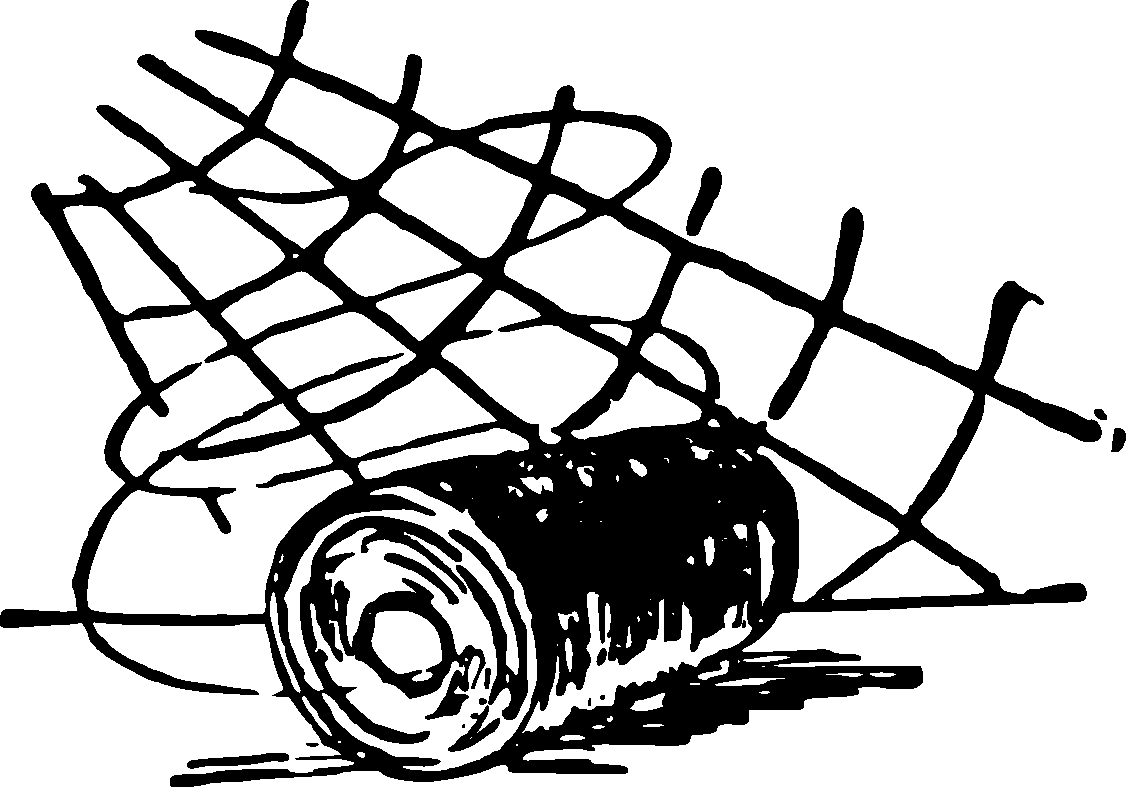
\includegraphics[width=0.3\textwidth]{figures/ch-11/fig-ch-11-tail.pdf}
\end{center}


















